% !TEX root=./chap-03-dummy.tex

\section{双杂化泛函的电性质梯度理论与程序实现}

\subsection{引言}

表征技术是实验科学问题的重要分支之一。对于化学而言,经典的红外 (IR, \underline{I}nf\underline{r}ared)、紫外或可见光 (UV-Vis, \underline{U}ltra-\underline{V}iolet and \underline{Vis}able)、拉曼 (Raman)、核磁 (NMR, \underline{N}uclear \underline{M}agnetic \underline{R}esonance) 等表征手段被合称为“四大光谱”\footnote{“四大光谱”的说法并不是正式的。也有将拉曼光谱替换为质谱 (MS, \underline{M}ass \underline{S}pectrometry) 或 X 射线衍射谱 (XRD, \underline{X}-\underline{R}ay \underline{D}iffraction) 等。正文中说道计算化学对谱学问题有所帮助;但并不是所有谱学问题都与电子结构有紧密的关系、基于第一性的计算化学也未必能解决或解释所有谱学问题。例如质谱与分子构型关联度更大、X 射线衍射与晶格本身更有关、通过计算化学难以给出色谱的保留时间等。},在以有机化学为代表的分支学科中是必要的佐证手段。近年来,扫描隧道显微镜 (STM, \underline{S}canning \underline{T}unneling \underline{M}icroscopy)、原位红外 (\emph{in situ} IR)、表面增强拉曼 (SERS, \underline{S}urface-\underline{E}nhanced \underline{R}aman \underline{S}catting/\underline{S}pectroscopy)、扫描电化学显微镜 (SEM, \underline{S}canning \underline{E}lectron \underline{M}icroscopy) 等众多新兴表征手段兴起。由于其中的许多表征问题可以归结为电子结构或分子振动效应,因此可以或有希望通过第一性的计算化学方法计算得到,从而实验与理论或计算可以相互印证,推动化学学科的发展。

在前几章中已经表明密度泛函方法,特别是双杂化密度泛函近似,在基态能量计算上有较好的表现。我们预期在谱学计算上,双杂化密度泛函方法也能有良好的表现。为此,我们需要发展双杂化泛函的谱学计算方法。由于较多光谱问题 (包括 IR、Raman、NMR 等) 可以归结为偶极电场或磁场 $\pmb{\mathcal{E}}$ 下平衡态分子的基态能量 $E(\pmb{\mathcal{E}})$ 扰动问题,其中 $\pmb{\mathcal{E}}$ 为微扰外场;那么光谱的强度经常取决于导数量
\begin{equation}
  \lim_{|\pmb{\mathcal{E}}| \rightarrow 0} \frac{\mathrm{d}^n E(\pmb{\mathcal{E}})}{\mathrm{d} \pmb{\mathcal{E}}^n}
\end{equation}
或其导出量、或多种外场下的混合导数量。光谱问题也经常与分子振动有关;若上式的外场 $\pmb{\mathcal{E}}$ 替换为原子坐标移动向量,那么分子振动将化归为 $n = 2$ 即二阶导数问题。对于这类光谱计算问题,为通过计算化学手段进行模拟,我们需要对能量在外场下的梯度理论作研究与程序化。我们也称可以化归为梯度计算的光谱或振动问题为\textsf{梯度性质}问题。

双杂化泛函的梯度性质已经有先驱性的程序实现与测评\cite{Neese-Grimme.JCP.2007, Biczysko-Barone.JCTC.2010, Su-Xu.JCC.2013, Stoychev-Neese.JCTC.2018, Gu-Xu.JCTC.2021, Yan-Xu.JCTC.2022}。这些工作表明,双杂化泛函,特别是 xDH 型泛函,在分子振动、NMR 光谱预测等问题上有优异的表现。但目前的程序在计算双杂化解析梯度问题上,效率还一定提升空间。同时,考虑到双杂化泛函除了 MP2 型相关能外还有其它的杂化可能性;在理论推导与程序化过程中,也应尽量留出空间以容纳其它杂化形式。

在本章工作中,基于前人的工作\cite{Gerratt-Mills.JCP.1968, Gerratt-Mills.JCP.1968a, Pople-Binkley.IJQC.1979, Dykstra-Jasien.CPL.1984, Handy-Schaefer.JCP.1984, Handy-Simandiras.CPL.1985, Pulay-Saeboe.TCA.1986, Trucks-Bartlett.CPL.1988, Frisch-Pople.CP.1990, Frisch-Pople.CPL.1990, Frisch-Pople.CPL.1990a, Gauss-Bartlett.JCP.1992, Stanton-Bartlett.CPL.1992, Johnson-Frisch.CPL.1993, Head-Gordon-Head-Gordon.CPL.1994, Yamaguchi-Schaefer.Oxford.1994, Weigend-Haeser.TCA.1997, Aikens-Gordon.TCA.2003, Cammi-Frisch.TCA.2004, Distasio-Head-Gordon.JCC.2007, Neese-Grimme.JCP.2007, Biczysko-Barone.JCTC.2010, Su-Xu.JCC.2013, Ji-Jung.JCTC.2013, Bykov-Neese.MP.2015, Stoychev-Neese.JCTC.2018, Gu-Xu.JCTC.2021, Yan-Xu.JCTC.2022},将以电性质外场微扰为前提下,进行双杂化二阶梯度梯度的理论推演、与基于原子轨道基的程序化。\ref{sec.3.background} 节将介绍物理问题背景与程序化背景,以确定大体的技术线路。\ref{sec.3.theory} 节将介绍一般双杂化泛函电性质解析梯度理论。MP2 型泛函作为双杂化泛函的其中一个重要的分支,其在 RI 近似下解析静态极化率的 Python 代码在 CPU 上的实现细节将在 \ref{sec.3.program} 阐述,并作简单的效率测评。

\subsection{背景:记号定义}

\subsubsection{Einstein 求和记号}

出于简化公式表达,后文将对张量缩并大量使用变种的 Einstein 求和记号 (Einstein notation)。一些例子是
\begin{subequations}
\begin{align}
  \label{eq.einsum.1}
  (ia|jb) = \sum_{\mu \nu \kappa \lambda} C_{\mu i} C_{\nu a} (\mu \nu | \kappa \lambda) C_{\kappa j} C_{\lambda b}
  &\Rightarrow 
  (ia|jb) = C_{\mu i} C_{\nu a} (\mu \nu | \kappa \lambda) C_{\kappa j} C_{\lambda b} \\
  \label{eq.einsum.2}
  E_\mathrm{c}^\textsf{(2)} = - \frac{1}{4} \sum_{iajb} \frac{\big| \langle i j || a b \rangle \big|^2}{\varepsilon_i + \varepsilon_j - \varepsilon_a - \varepsilon_b}
  &\Rightarrow
  E_\mathrm{c}^\textsf{(2)} = - \frac{1}{4} \frac{\big| \langle i j || a b \rangle \big|^2}{\varepsilon_i + \varepsilon_j - \varepsilon_a - \varepsilon_b} \\
  \label{eq.einsum.3}
  \rho_g = \sum_{\mu \nu} D_{\mu \nu} \phi_{g \mu} \phi_{g \nu}
  &\Rightarrow
  \rho_g = D_{\mu \nu} \phi_{g \mu} \phi_{g \nu} \\
  \label{eq.einsum.4}
  L_{ai}^\textsf{xDH} = - (\varepsilon_a - \varepsilon_i) Z_{ai}^\textsf{xDH} - \sum_{bj} A_{ai, bj} Z_{bj}^\textsf{xDH}
  &\Rightarrow
  L_{ai}^\textsf{xDH} = - (\varepsilon_a - \varepsilon_i) Z_{ai}^\textsf{xDH} - A_{ai, bj} Z_{bj}^\textsf{xDH}
\end{align}
\end{subequations}
需要指出,这里的 Einstein 求和记号与物理中通常使用的记号不同\cite{Einstein-Einstein.AP.1916}。在物理中的 Einstein 求和记号依据对偶空间分上下标;以式 (\ref{eq.einsum.1}) 为例,若记 $g_{ij}^{ab} = (ia|jb)$,则通常物理的 Einstein 求和应写为:
\begin{equation*}
  g_{ij}^{ab} = C^\mu_i C^a_\nu g^{\nu \lambda}_{\mu \kappa} C^\kappa_j C^b_\lambda
\end{equation*}
物理中的 Einstein 求和,会将等式一侧任何重复出现的角标进行求和;但对于式 (\ref{eq.einsum.3}, \ref{eq.einsum.4}),我们所使用的变种的 Einstein 求和记号的等式右出现重复了两次的角标但并未被求和,而是对角标作元素乘法 (elementwise multiplication)。对于式 (\ref{eq.einsum.3}),角标 $g$ 并不处于 $\mu, \nu$ 所在的对偶空间,因此没有物理中 Einstein 记号的对应写法。对于式 (\ref{eq.einsum.4}),由于我们一般要求自洽场计算是正则的 (canonical),即 Fock 矩阵 $F_{pq}$ (或依物理的 Einstein 记号记为 $F_p^q$) 是对角矩阵且其对角元 $\varepsilon_p$ 被称为轨道能;因此式 (\ref{eq.einsum.4}) 在物理的 Einstein 记号下是
\begin{equation*}
  (L_a^i){}^\textsf{(2)} = - F_a^b (D_b^i){}^\textsf{(2)} - F_j^i (D_a^j){}^\textsf{(2)} - A_{aj}^{ib} (D_b^j){}^\textsf{(2)}
\end{equation*}
本文档的公式所使用的变种 Einstein 求和记号,会比较接近于具体程序实现时的情形 (\verb|NumPy.einsum| 或 \verb|opt_einsum.contract|),并允许打破一些物理记号的限制。

\subsubsection{记号与角标}

本工作通常使用下述记号:
\begin{itemize}[nosep]
  \item 下标 $\mu, \nu, \kappa, \lambda, \eta, \xi$:原子轨道 (基轨道);
  \item 下标 $i, j, k, l$:占据分子轨道;
  \item 下标 $a, b, c$:非占分子轨道;
  \item 下标 $p, q, r, s, m$:任意分子轨道;
  \item 下标 $P, Q, R, S$:RI 辅助基轨道;
  \item 上下标 $\mathbb{A}, \mathbb{B}$:外场微扰量、被求导量;
  \item 下标或向量 $A, B, M$:原子核;
  \item 下标 $w, t$:坐标分量 (用于指代 $x, y, z$);
  \item 下标 $\rho, \gamma$:密度与梯度导出量;
  \item 上标 $\mathrm{n}$:非变分泛函 (\underline{N}on-variational,相对于自洽场泛函);
  \item 上标 $\mathrm{S}$:\underline{S}keleton 导数;
  \item 上标 $\mathrm{U}$:轨道旋转导数 (\underline{U}nitary Transformation,涉及 U 矩阵 (\ref{eq.def.U}) 的导数);
  \item 上标 $\sigma, \varsigma$:自旋 (指代 $\alpha$ 或 $\beta$);
  \item 临时记号 $\mathscr{T}$ 作为算法中间张量,仅在局部的前后文中有意义。
\end{itemize}

本工作在不作额外说明的情形时,将讨论闭壳层 (closed-shell) 实现;对于开壳层问题,不同自旋下的轨道通过上标横线区分 ($p$ 表示 $\alpha$ 自旋、$\bar p$ 表示 $\beta$ 自旋),矩阵或张量则将上标具体的自旋。

本工作的全部理论推导与程序实现使用实数。为简化公式表达,大多数情形将不使用复共轭记号 (上标星号 $*$)。通常使用 $\phi_\mu (\bm{r})$ 表示原子轨道 $\mu$ 在空间坐标 $\bm{r}$ 下的函数表达式。对于 DFT 格点积分,若记坐标在角标 $g$ 下的离散格点为 $\bm{r}_g$,那么也经常用 $\phi_{g \mu}$ 作为二阶张量表示空间格点下的原子轨道函数值 $\phi_\mu (\bm{r}_g)$。

\subsubsection{部分常用表达式}

本工作使用到的电子积分有:
\begin{itemize}[nosep]
  \item 重叠积分 $S_{\mu \nu}$ (overlap):
        \begin{equation}
          S_{\mu \nu} := \int \phi_\mu (\bm{r}) \phi_\nu (\bm{r}) \, \mathrm{d} \bm{r}
        \end{equation}
  \item 无外场下的外势积分 $V_{\mu \nu}$:
        \begin{equation}
          V_{\mu \nu} := \int \phi_\mu (\bm{r}) \frac{- Z_A}{|\bm{r} - \bm{A}|} \phi_\nu (\bm{r}) \, \mathrm{d} \bm{r}
        \end{equation}
        上式对原子核角标 $A$ 求和;$Z_A$ 是原子单位下的原子核电荷数。
  \item 无外场下单电子积分 $h_{\mu \nu}$ (Hamiltonian core):
        \begin{equation}
          h_{\mu \nu} := S_{\mu \nu} + V_{\mu \nu}
        \end{equation}
  \item 四中心双电子互斥积分 $(\mu \nu | \kappa \lambda)$ (4c-2e ERI, 4-\underline{c}enter 2-\underline{e}lectron \underline{E}lectron \underline{R}epulsion \underline{I}ntegral):
        \begin{equation}
          (\mu \nu | \kappa \lambda) := \iint \phi_\mu (\bm{r}_1) \phi_\nu (\bm{r}_1) \frac{1}{r_{12}} \phi_\kappa (\bm{r}_2) \phi_\lambda (\bm{r}_2) \, \mathrm{d} \bm{r}_1 \mathrm{d} \bm{r}_2
        \end{equation}
        该积分也称传统双电子积分 conventional ERI 或简记为 conv ERI。
  \item 三中心双电子互斥积分 $(\mu \nu | P)$ (3c-2e ERI):
        \begin{equation}
          (\mu \nu | P) := \iint \phi_\mu (\bm{r}_1) \phi_\nu (\bm{r}_1) \frac{1}{r_{12}} \phi_P (\bm{r}_2) \, \mathrm{d} \bm{r}_1 \mathrm{d} \bm{r}_2
        \end{equation}
  \item 双中心双电子互斥积分 $J_{PQ}$ (2c-2e ERI):
        \begin{equation}
          J_{PQ} := \iint \phi_P (\bm{r}_1) \frac{1}{r_{12}} \phi_Q (\bm{r}_2) \, \mathrm{d} \bm{r}_1 \mathrm{d} \bm{r}_2
        \end{equation}
\end{itemize}

除了密度矩阵、弛豫张量等情形外,其它的原子轨道基下的张量,转换到分子轨道基时总是乘以轨道系数矩阵 $C_{\mu p}$。以原子与分子轨道混合基下的三中心双电子积分 $(\mu i | P)$ 为例,
\begin{equation*}
  (\mu i | P) = (\mu \nu | P) C_{\nu i}
\end{equation*}

在不引起歧义的情况下,将使用矩阵或张量元素指代矩阵或张量本身,例如用 $D_{\mu \nu}$ 表示完整的自洽场密度矩阵 $\mathbf{D}$。

本工作常用到的表达式有
\begin{itemize}[nosep]
  \item 闭壳层自洽场密度矩阵 $D_{\mu \nu}$ 与 $D_{pq}$:
        \begin{alignat}{10}
          \label{eq.def.dm-scf-closed}
          D_{\mu \nu} &:= C_{\mu p} D_{pq} C_{\nu q} = 2 C_{\mu i} C_{\nu i} \quad &&\text{(closed-shell)} \\
          D_{pq} &:= 2 \delta_{pq} \delta_{p \in \mathrm{occ}} \quad &&\text{(closed-shell)}
        \end{alignat}
        上式的 $\delta_{p \in \mathrm{occ}}$ 是指当 $p$ 属于占据轨道时取 1、不属于占据轨道时取 0。后文将涉及其它类型的密度 (譬如 xDH 约化密度 $D_{pq}^{\textsf{xDH}, \textsf{RDM}}$ 与弛豫密度 $D_{pq}^{\textsf{xDH}}$),需要上标类型以作区分;除自旋记号、没有额外上标的密度,均视为自洽场密度。
  \item 开壳层自洽场密度矩阵 $D_{\mu \nu}^\alpha$ 与 $D_{pq}$:
        \begin{align}
          D_{\mu \nu}^\alpha &:= C_{\mu p} D_{pq} C_{\nu q} = C_{\mu i} C_{\nu i} \\
          D_{pq} &:= \delta_{pq} \delta_{p \in \mathrm{occ}}
        \end{align}
        对于 $\beta$ 自旋的情形是类似的:
        \begin{align}
          D_{\mu \nu}^\beta &:= C_{\mu \bar p} D_{\bar p \bar q} C_{\nu \bar q} = C_{\mu \bar i} C_{\nu \bar i} \\
          D_{\bar p \bar q} &:= \delta_{\bar p \bar q} \delta_{\bar p \in \mathrm{occ}}
        \end{align}
        开壳层自洽场的总密度矩阵记为 $D_{\mu \nu} = D_{\mu \nu}^\alpha + D_{\mu \nu}^\beta$。
  \item 双杂化泛函总能量 $E^\textsf{tot}$:
        \begin{equation}
          \label{eq.def-E-tot}
          E^\textsf{tot} := E^\textsf{core} [\mathbf{D}] + E^\textsf{ERI} [\mathbf{D}] + E^\textsf{DFA} [\mathbf{D}] + E^\textsf{PT} [\mathbf{C}] + E^\textsf{non-elec} \\
        \end{equation}
        对于杂化泛函,$E^\textsf{PT} [\mathbf{C}]$ 取零值。每个能量分项的计算将在下面列举。需要指出,上式表述的是目前流行的双杂化泛函的能量表达式,而并非定义式。
  \item 单电子积分能量 $E^\textsf{core} [\mathbf{D}]$:
        \begin{equation}
          E^\textsf{core} [\mathbf{D}] := h_{\mu \nu} D_{\mu \nu}
        \end{equation}
  \item 双电子积分能量 $E^\textsf{ERI} [\mathbf{D}]$:
        \begin{equation}
          \label{eq.def.eng-eri}
          E^\textsf{ERI} [\mathbf{D}] := E^\textsf{J} [\mathbf{D}] + c_\mathrm{x} E_\mathrm{x}^\textsf{exact} [\mathbf{D}] + c_\mathrm{x}^\textsf{LR} E_\mathrm{x}^\textsf{LR} [\mathbf{D}]
        \end{equation}
        其中,$E^\textsf{J} [\mathbf{D}]$ 是库伦能\footnote{事实上,尽管本工作对双电子积分 $(\mu \nu | \kappa \lambda)$ 作近似;但该近似是 \ref{sec.rijk-rimp2-efficiency} 小节 RI 近似,它使用了计算复杂度为 $O(n_\mathrm{AO}^2 n_\mathrm{aux}) \sim O(N^3)$ 的三中心双电子积分 $(\mu \nu | P)$,因而在实际程序中仍然使用密度矩阵 $\mathbf{D}$ 描述库伦能。库伦能在程序实现上,确实可以通过密度格点 $\rho$ 而非具有更多细节的密度矩阵 $\mathbf{D}$ 计算实现、且计算复杂度为更小的 $O(N^2)$\cite{Toivanen-Sundholm.PCCP.2015};但我们的主要研究对象是双杂化泛函,在交换能 $E_\mathrm{x}^\textsf{exact}$ 与微扰能 $E^\textsf{PT}$ 难以使用密度格点 $\rho$ 进行计算的情况下,在程序实现中使用密度矩阵 $\mathbf{D}$ 以描述库伦能相信是可以接受的。}
        \begin{equation}
          \label{eq.def.ej}
          E^\textsf{J} [\mathbf{D}] = J[\rho] := \frac{1}{2} D_{\mu \nu} (\mu \nu | \kappa \lambda) D_{\kappa \lambda}
        \end{equation}
        $c_\mathrm{x}$ 特指严格交换系数 (区别于其它 DFA 交换系数),$E_\mathrm{x}^\textsf{exact} [\mathbf{D}]$ 是严格交换能
        \begin{equation}
          E_\mathrm{x}^\textsf{exact} [\mathbf{D}] = E_\mathrm{x}^\textsf{exact} [\rho] := - \frac{1}{2} D_{\mu \nu}^\sigma (\mu \lambda | \kappa \nu) D_{\kappa \lambda}^\sigma
        \end{equation}
        对于闭壳层问题,严格交换能可以写为
        \begin{equation}
          E_\mathrm{x}^\textsf{exact} [\mathbf{D}] := - \frac{1}{4} D_{\mu \nu} (\mu \lambda | \kappa \nu) D_{\kappa \lambda} \quad \text{(closed-shell)}
        \end{equation}
        部分泛函在交换能部分考虑了长短程效应;长程 (LR, \underline{L}ong-\underline{R}ange) 部分能量 $E_\mathrm{x}^\textsf{LR}$ 的双电子除了积分算符通常是 $\mathrm{erf} (\mu r_{12}) / r_{12}$\footnote{$\mu$ 是长程矫正的参数,通常小于 1。对于长程矫正作用,使用误差函数 $\mathrm{erf} (\mu r_{12}) / r_{12}$ 是常见且最多程序实现的方法;但除此之外,Yukawa 衰减算符 $\mathrm{exp} (-\mu r_{12}) / r_{12}$\cite{Savin-Flad.IJQC.1995} 与 $\mathrm{terf}$ 函数 $$\mathrm{terf} (r, r_0) := \frac{1}{2} \left( \mathrm{erf} \left(\frac{r - r_0}{\sqrt{2} r_0}\right) + \mathrm{erf} \left(\frac{r + r_0}{\sqrt{2} r_0}\right) \right)$$ 所构成的衰减算符 $\mathrm{terf} (-\mu r_{12}) / r_{12}$\cite{Goldey-Head-Gordon.PCCP.2013},也是其它可能使用到的长程矫正方案。},在计算、程序调用、张量分解等具体的程序实现上等同于严格交换能 $E_\mathrm{x}^\textsf{exact}$\footnote{需要指出,这只是双电子能量积分的一种表达方法。以 Cammi 等\cite{Cammi-Frisch.TCA.2004}对溶剂化模型下 MP2 二阶梯度理论为例,该文将电子效应诱导的溶剂化能量与双电子积分能量合并处理;而溶剂化能量的计算本身是不具有双电子积分。同时,在以较为抽象的层面上推导二阶梯度问题时,DFA 格点积分能量 $E^\textsf{DFA} [\mathbf{D}]$ 与双电子积分有类似的推演过程;因此从梯度理论的角度来讲,拆分双电子积分能量 $E^\textsf{ERI}$ 与 DFA 格点积分能量 $E^\textsf{DFA}$ 是人为的。在本工作中,我们不涉及溶剂化、基于密度的长程弥散矫正等其它无法简单纳入单电子积分能量的贡献;因此从程序实现方便、或计算量差异的角度,拆分了双电子积分能量与 DFA 格点积分能量。}。
  \item DFA 格点积分能量 $E^\textsf{DFA} [\mathbf{D}]$\footnote{区别于 DFA 近似总能量 $E^\textsf{tot}$。} 用以处理“Jacob 阶梯”上 1--3 阶 (LDA, GGA, meta-GGA) 交换相关能;它可以表示为对空间的积分
        \begin{equation}
          E^\textsf{DFA} [\mathbf{D}] := \int f[\rho, \gamma, \tau, \nabla^2 \rho, \cdots] \rho \, \mathrm{d} \bm{r}
        \end{equation}
        上式的 $f$ 若看作关于电子坐标 $\bm{r}$ 的函数,则其物理意义是在 $\bm{r}$ 处每个电子所具有的能量分布。$f$ 的具体表达式,取决于不同密度泛函所作不同的近似。其中,$\gamma$ 为 GGA 所用到的密度梯度导出量
        \begin{equation}
          \gamma := \nabla \rho \cdot \nabla \rho
        \end{equation}
        需要指出,动能密度 $\tau$ 导出自 Kohn-Sham 占据轨道 $\phi_i$ 而非密度 $\rho$ 本身,从而 $\tau$ \alert{引用第一章公式} 需要通过密度矩阵 $\mathbf{D}$、而非密度 $\rho$ 导出\footnote{对于 GGA 与 LDA,其能量或高阶导数确实是通过密度格点 $\rho$ 本身导出。以密度矩阵 $\mathbf{D}$ 作为参数不影响后文讨论;见库伦能定义式 (\ref{eq.def.ej}) 的脚注。}。因此在本工作中,为容许 meta-GGA 的程序实现,我们将 $E^\textsf{DFA}$ 视作密度矩阵 $\mathbf{D}$ 的泛函。在程序实现中,空间积分将化为格点积分求和式:
        \begin{equation}
          E^\textsf{DFA} \simeq w_g f_g \rho_g
        \end{equation}
        其中,$w_g$ 是空间坐标 $\bm{r}_g$ 下的格点积分权重、$f_g$ 与 $\rho_g$ 是能量分布函数与电子云密度在空间坐标 $\bm{r}_g$ 下的数值。
  \item 微扰能量 $E^\textsf{PT}[\mathbf{C}]$ 是双杂化泛函中的高阶近似部分。由于目前流行的杂化形式是 MP2 型相关能,因此这里统称为微扰能;但它也可以代表 IEPA 型相关能、RPA 型相关能等其它种类能量贡献项。一般来说,微扰能量 $E^\textsf{PT}$ 不纳入自洽场计算中,且并非密度矩阵 $\mathbf{D}$ 而是作为自洽场结果的轨道系数 $\mathbf{C}$ 的泛函。
  \item 无外场下的非电子效应能量 $E^\textsf{non-elec}$:
        \begin{equation}
          E^\textsf{non-elec} := \frac{1}{2} \frac{Z_A Z_B}{r_{AB}}
        \end{equation}
        其中,距离 $r_{AB}$ 定义为
        \begin{equation*}
          r_{AB} :=
          \begin{cases}
              | \boldsymbol{A} - \boldsymbol{B} | & A \neq B \\
              + \infty & A = B
          \end{cases}
        \end{equation*}
\end{itemize}

\subsubsection{xDH 型自洽场泛函与能量泛函}

xDH 型泛函分别对自洽场与总能量使用两种泛函形式;我们分别称之为\textsf{自洽场泛函}与\textsf{能量泛函}。由于 xDH 型泛函最终的能量并非通过变分得到,我们也称能量泛函为非变分泛函。自洽场是对下述能量求取分子轨道系数 $C_{\mu i}$ 的变分极小得到:
\begin{equation}
  \label{eq.def.eng-SCF}
  E^\textsf{SCF} = E^\textsf{core} [\mathbf{D}] + E^\textsf{ERI} [\mathbf{D}] + E^\textsf{DFA} [\mathbf{D}] + E^\textsf{non-elec}
\end{equation}
能量泛函部分项使用上标 $\mathrm{n}$ 进行区分;将自洽场给出的分子轨道系数 $C_{\mu p}$ 代入下式得到 xDH 能量:
\begin{equation}
  \label{eq.def.eng-xDH}
  E^\textsf{xDH} = E^\textsf{core} [\mathbf{D}] + E^{\mathrm{n}, \textsf{ERI}} [\mathbf{D}] + E^{\mathrm{n}, \textsf{DFA}} [\mathbf{D}] + E^\textsf{PT} [\mathbf{C}] + E^\textsf{non-elec}
\end{equation}
其中,$E^\textsf{core} [\mathbf{D}]$ 与 $E^\textsf{non-elec}$ 对于能量泛函和自洽场泛函没有区别。微扰能 $E^\textsf{PT} [\mathbf{C}]$ 仅在能量泛函出现;出于行文便利,将不对其作 $\mathrm{n}$ 的上标区分。为了后文讨论上的方便,我们额外定义 $E^{\mathrm{n}, \textsf{hyb}}$ 作为 $E^\textsf{xDH}$ 中,仅与密度矩阵 $\mathbf{D}$ 依赖的所有项之和:
\begin{equation}
  \label{eq.def.eng-n-hyb}
  E^{\mathrm{n}, \textsf{hyb}} := E^\textsf{core} [\mathbf{D}] + E^{\mathrm{n}, \textsf{ERI}} [\mathbf{D}] + E^{\mathrm{n}, \textsf{DFA}} [\mathbf{D}]
\end{equation}

需要补充的是,bDH 型泛函是当 xDH 型泛函的 $E^{\mathrm{n}, \textsf{ERI}} = E^\textsf{ERI}$、$E^{\mathrm{n}, \textsf{DFA}} = E^\textsf{DFA}$ 时的退化版本。bDH 型泛函由于仍然存有 $E^\textsf{PT} [\mathbf{C}]$ 一项,因此总能量泛函与 xDH 同样都是通过非变分途径计算得来。在目前的程序实现上,我们不需要区分 bDH 与 xDH 两者。

\subsubsection{导数记号与耦合微扰}

本工作将依是否存在耦合微扰 (CP, \underline{C}oupled \underline{P}erturbed),分为 Skeleton 导数 (骨架导数,部分文献也称为 core 导数即核导数)、轨道旋转导数、与一般的全导数。对于导数记号,在不引起歧义的情况下,
\begin{itemize}[nosep]
  \item 以分数形式描述的导数,$\frac{\mathrm{d}}{\mathrm{d} \mathbb{A}}$ 表示全导数,$\frac{\partial}{\partial \mathbb{A}}$ 表示偏导数;
  \item 以简写形式描述的导数,$\partial_\mathbb{A}$ 记号是\textsf{全导数} $\frac{\mathrm{d}}{\mathrm{d} \mathbb{A}}$ 的简记 (并非偏导数的含义,这是为了字母 $\mathrm{d}$ 被认为是变量);对性质量 $\mathbb{A}$ 的偏导数称为 Skeleton 导数并记为 $\partial_\mathbb{A}^\mathrm{S}$;涉及轨道系数的导数记为 $\partial_\mathbb{A}^\mathrm{U}$。$\partial_\mathbb{A}^\mathrm{S}$ 与 $\partial_\mathbb{A}^\mathrm{U}$ 将在这一小节的后文定义。
\end{itemize}

以总能量为例,在\textsf{特定的}外加微扰 $\mathbb{A}$ 与轨道系数 $\mathbf{C}$ 下,其能量记为 $E^\textsf{xDH} (\mathbb{A}, \mathbf{C})$。对于 xDH 型泛函,轨道系数是通过自洽场泛函得到;该轨道系数是随外加微扰而变化的\footnote{在本工作中,我们假定轨道系数随外加微扰是可以变化的,进而定义 U 矩阵 (\ref{eq.def.U}) 以描述轨道扰动情况\cite{Handy-Schaefer.JCP.1984}。尽管这一小节明确分别定义了对微扰外场与对分子轨道的偏导数,但当能量项的计算比较复杂时、或导数阶数高时,分子轨道系数对微扰外场的依赖性会增加推导难度。

另一类做法是完全避免使用 U 矩阵,而将轨道系数 $C_{\mu p}$、自洽场方程 (\ref{eq.SCF-working-equation}) 的 Lagrange 乘子 $\varepsilon_{pq}$、弛豫密度矩阵 $D_{pq}^\textsf{xDH}$ 作为自洽场方程 (\ref{eq.SCF-working-equation}) 的 Lagrange 乘子、加权密度矩阵 $W_{pq}^\textsf{xDH}$ 作为正交条件 (\ref{eq.constraint.ortho}) 的 Lagrange 乘子,这些变量都作为新构造的 Lagrangian 的参数;从而对该 Lagrangian 作梯度推演\cite{Helgaker-Joergensen.TCA.1989, Burow-Eshuis.JCTC.2014}。通过这个大量利用 Lagrange 乘子的方法,弛豫密度与能量加权密度矩阵都是自然定义的,而不需要像本工作以 Skeleton 梯度 (\ref{eq.collary.rdm-definition}) 定义 (难以通过波函数确定的、非变分方法的) 约化密度、以 Z-Vector 方程 (\ref{eq.Z-vector}) 进一步定义弛豫密度这样绕弯子的做法。同时,该推导途径也不需要特意引入作为数学技巧的 Z-Vector 方法 (\ref{eq.Z-vector-contrib-to-eng-deriv}) 与交换定理 (\ref{eq.interchange-theorem});且不需要考虑因轨道能级简并,而产生在强的正则自洽场条件 (\ref{eq.constraint.canonical-SCF}) 下,U 矩阵部分矩阵元数值不稳定的情形 (\ref{eq.unstable-Uij})。但该推导途径在目前大量涉及 MP2 型相关能的二阶梯度推演与计算中不是主流,且不会因其推演方式不同而给出更简洁或更高效的公式与程序;因此我们的工作仍然依主流的方法,使用 U 矩阵。\label{footnote.full-lagrangian}}:
\begin{equation*}
  \mathbf{C}^\textsf{SCF} (\mathbb{A}) := \arg \min_\mathbf{C} E^\textsf{SCF} (\mathbb{A}, \mathbf{C}) \quad \text{(with eq (\ref{eq.constraint.ortho}) satisfied)}
\end{equation*}
从而,实际的 xDH 能量不仅受外加微扰 $\mathbb{A}$ (作为函数 $E^\textsf{xDH} (\mathbb{A}, \mathbf{C})$ 的变量参数第一项) 而产生变化,同时轨道系数 $\mathbf{C}^\textsf{SCF} (\mathbb{A})$ (作为变量参数的第二项) 也受外加微扰 $\mathbb{A}$ 的耦合扰动;因此准确地来说,xDH \textsf{基态能量}应写为 $E^\textsf{xDH} (\mathbb{A}, \mathbf{C}^\textsf{SCF} (\mathbb{A}))$。由于我们总是处理基态的能量与梯度计算问题,因此后文默认轨道系数 $\mathbf{C}$ 是自洽场变分极小的 $\mathbf{C}^\textsf{SCF}$。

为讨论问题的方便,定义 Skeleton 导数为轨道系数未耦合扰动下的导数。以 xDH 能量为例,
\begin{equation}
  \partial_\mathbb{A}^\mathrm{S} E^\textsf{xDH} := \frac{\partial E^\textsf{xDH} (\mathbb{A}, \mathbf{C} (0))}{\partial \mathbb{A}}
\end{equation}
为与一般的全导数作区分,Skeleton 导数使用记号 $\partial_\mathbb{A}^\mathrm{S}$,即上标 $\mathrm{S}$。同时,我们定义轨道旋转导数
\begin{equation}
  \partial_\mathbb{A}^\mathrm{U} E^\textsf{xDH} := \frac{\partial E^\textsf{xDH} (\mathbb{A}, \mathbf{C})}{\partial \mathbf{C}} \frac{\partial \mathbf{C} (\mathbb{A})}{\partial \mathbb{A}}
\end{equation}
我们使用 $\partial_\mathbb{A}^\mathrm{U}$,即上标 $\mathrm{U}$,表示轨道旋转导数。

进而,xDH 能量的全导数,依据求导规则,它等于 Skeleton 导数与对轨道系数导数的和:
\begin{equation}
  \partial_\mathbb{A} E^\textsf{xDH} = \partial_\mathbb{A}^\mathrm{S} E^\textsf{xDH} + \partial_\mathbb{A}^\mathrm{U} E^\textsf{xDH}
\end{equation}

除能量外,上述导数记号对其它标量或张量也成立。以分子轨道基下单电子积分矩阵 $h_{pq}$ 导数为例,
\begin{equation*}
  h_{pq} = C_{\mu p} h_{\mu \nu} C_{\nu q}
\end{equation*}
注意到原子轨道基下 $h_{\mu \nu}$ 没有分子轨道系数的参与,因此 Skeleton 导数是
\begin{equation*}
  h_{pq}^\mathbb{A} := \partial_\mathbb{A}^\mathrm{S} h_{pq} := C_{\mu p} \frac{\partial h_{\mu \nu}}{\partial \mathbb{A}} C_{\nu q}
\end{equation*}
而轨道系数导数为
\begin{equation*}
  \partial_\mathbb{A}^\mathrm{U} h_{pq} := \frac{\partial C_{\mu p}}{\partial \mathbb{A}} h_{\mu \nu} C_{\nu q} + C_{\mu p} h_{\mu \nu} \frac{\partial C_{\nu q}}{\partial \mathbb{A}}
\end{equation*}
全导数为上述三项之和:
\begin{align*}
  \partial_\mathbb{A} h_{pq} &= \partial_\mathbb{A}^\mathrm{S} h_{pq} + \partial_\mathbb{A}^\mathrm{U} h_{pq} \\
  &= \frac{\partial C_{\mu p}}{\partial \mathbb{A}} h_{\mu \nu} C_{\nu q} + C_{\mu p} \frac{\partial h_{\mu \nu}}{\partial \mathbb{A}} C_{\nu q} + C_{\mu p} h_{\mu \nu} \frac{\partial C_{\nu q}}{\partial \mathbb{A}} \\
  &= \frac{\partial C_{\mu p}}{\partial \mathbb{A}} \frac{\partial h_{pq}}{\partial C_{\mu p}} + h_{pq}^\mathbb{A} + \frac{\partial h_{pq}}{\partial C_{\nu q}} \frac{\partial C_{\nu q}}{\partial \mathbb{A}}
\end{align*}


\subsection{背景:物理背景与程序化}
\label{sec.3.background}

\subsubsection{Python 相关背景}

本工作的程序实现化完全使用 Python 实现。

第一性计算化学的程序化问题,通常涉及到大量的浮点运算与内存调用,对程序性能的效率要求相当高。因此,目前计算化学程序通常使用效率较高的编译语言。计算化学尽管存在商业化前景,但受益的受众较小、并非民生或娱乐所必须;因此程序开发对化学工作者之外的人才吸引力有限。计算化学软件的开发由于专业性要求高、公式较复杂、模块化较困难,因此存在程序开发与管理上的难度。这些特性使得曾经与当前的计算化学程序开发周期较长,因此现在流行的计算化学软件通常都使用 1960 年代发展至今的 Fortran 语言 (包括但不限于 Gaussian、ORCA、VASP、NWChem、CP2K、Quantum ESPRESSO、GAMESS-US、TurboMole、Molpro、CFOUR、MRCC、FHI-Aims、BDF)。

早期发展的 Fortran 与 C 等编译语言,其程序可读性与可复用性、安全性、可扩展性通常较差。为解决这些困难,计算机工作者开发了众多新型的编译语言,譬如 C++ 或 Rust。基于这类新的编译语言,Q-Chem (Fortran、C、C++ 混合)、Psi4 (C++、Python 混合)、ABACUS (C++)、REST (Rust) 得以开发。这类编译语言尽管运行耗时通常较低,但通常编译与调试耗时较长;同时语言的学习成本较高。类如 Java、C\# 等语言通过引入虚拟机而有较低的编译耗时;但这类语言的设计初衷大多并非科学计算、而更着重窗体设计与并发,因此这些语言的科学计算生态不太完整。

以 Python、Julia 为代表的语言与传统的编译或基于虚拟机的语言有许多不同。这类语言作为脚本或类脚本的语言,程序在编写时就能运行得到结果,这可以大幅加快程序开发周期;同时不需要严格的类型推断,因此这类语言从设计上就是泛型的,且便于对于复杂多变的条件判断或程序流程设计;但这经常以牺牲代码安全性为代价。对于 Python,尽管它不具有函数重载 (overload) 等功能,但具有绝大多数现代程序设计的要素,譬如类、继承与虚函数、文件模块化、属性、修饰等;因此可以很好地应对绝大多数业务逻辑。同时,由于 Python 在语言发展的早期搭建了 PyPI (\underline{Py}thon \underline{P}ackage \underline{I}ndex),有良好的程序生态与开源社群,帮助众多程序设计者借用其它人的工作,快速搭建程序。

Python 在性能上的缺陷,特别是 for 循环的效率问题,是众所周知的。这意味着仅使用 Python 语言特性本身,无法实现高性能运算。但 Python 允许使用封装 C、C++、Fortran 等其它语言所编译得到的程序库。以 NumPy、SciPy、Numba、PyTorch、Jax 为代表的高性能数学库或接口是基于 C++ 底层实现编写而来;如果一些计算特性难以通过通用数学库实现,Python 也允许用户自行编写并编译 C、C++、Fortran 库函数,使用 ctypes、pybind11、f2py 等库调用这些库。Psi4NumPy 等程序作为雏形软件与教程,有效地将 Python 高计算效率与开发效率引入到计算化学中。PySCF 作为计算化学软件,在程序的业务逻辑上完全以 Python 实现;但在具体的计算密集问题上,在性能损耗不严重的情形下使用纯 Python,而性能关键的代码则用 NumPy、SciPy 或 C 程序结合 ctypes 调用。在合理的算法支持下,基于 Python 的程序仍然可以达到相当高的计算效率。

第一性计算化学,特别是 post-HF 方法和梯度性质计算问题,经常可以化归为多步张量缩并 (tensor contraction) 问题。张量缩并本身经常也可以化归为张量转置合并矩阵计算问题。尽管已经有高效率的库函数用以实现张量转置 (以 HPTT 为代表) 与矩阵乘法 (以 BLAS 为基础的各数学库),但一方面这种拆分会将程序逻辑复杂化,降低开发效率;另一方面张量转置本身是访存密集型问题从而难以有高并行效率与高速缓存利用率、且不产生有效的浮点运算 (FLOPs, \underline{Fl}oating-point \underline{Op}eration\underline{s}),因此张量缩并分解为转置与乘法的方法不一定能发挥最高的浮点运算效率 (FLOPS, \underline{Fl}oating-point \underline{O}perations \underline{P}er \underline{S}econd)。因此,以 TBLIS、opt\_einsum 为代表的众多工作直接实现张量缩并,避免转置对 FLOPS 的浪费,且实现了简单易用的函数签名。这些程序在以四中心双电子的积分转换为代表的访存计算混合型问题中
\begin{equation*}
  (ia|jb) = \sum_{\mu \nu \kappa \lambda} C_{\mu i} C_{\nu a} (\mu \nu | \kappa \lambda) C_{\kappa j} C_{\lambda b}
\end{equation*}
有良好的表现;但这类程序作为通用张量缩并的优化,对特化的缩并问题不一定能提供最高的优化效率。PySCF 中,不需要额外调用转置的乘法问题将使用 NumPy 的矩阵乘法、复杂的张量缩并调用 TBLIS 实现、访存密集的问题使用 \verb|numpy.einsum| 实现。在我们当前对双杂化泛函的梯度实现中,为编写程序上的便利,将大量使用 PySCF 封装的 TLIBS 接口。

\subsubsection{RI 近似、RI-JK 与 RI-MP2 程序化与效率测试}
\label{sec.rijk-rimp2-efficiency}

这一节将引入 RI (\underline{R}esolution of \underline{I}dentity 或 Density Fitting) 近似;并通过简单的程序实现与效率测试,表明仅使用 Python 编写程序,充分利用现有的 Python 库函数,在内存充足的单节点 CPU 前提下,至少对于 RI-MP2 的相关能 $E_\mathrm{c}^\textsf{(2)}$ 计算,其程序效率可以不亚于流行的计算化学软件。

不论是 Hartree-Fock、密度泛函或 post-HF 方法,都需要在计算中使用双电子互斥算符 $1 / r_{12} = 1 / |\bm{r}_1 - \bm{r}_2|$。在原子轨道表示下,通常使用传统双电子积分 4c-2e ERI $(\mu \nu | \kappa \lambda)$ 展开该算符。由于 Hartree-Fock 或密度泛函的自洽场计算中,涉及 ERI 的部分相当耗时,且为 $O(n_\mathrm{basis}^4)$ 计算复杂度。

为降低电子积分部分的计算量,基于 Friesner 的伪谱法对电子积分的尝试\cite{Friesner-Friesner.CPL.1985, Friesner-Friesner.JCP.1987},Vahtras、Alml\"of、Feyereisn 等人具体地提出了分解 4c-2e ERI 到 3c-2e ERI 与 2c-2e ERI 或双中心重叠积分的三种策略 (SVS, S, V)\cite{Vahtras-Feyereisen.CPL.1993}。目前广为使用的策略是 V 策略,也称为 RI-V (\underline{R}esolution-of-\underline{I}dentity V):
\begin{equation}
  (\mu \nu | \kappa \lambda) := (\mu \nu | P) (\mathbf{J}^{-1})_{PQ} (\kappa \lambda | Q) \quad \text{(RI-V)}
\end{equation}
后文所有 RI 均默认是 RI-V 模式。

以 RI 近似计算自洽场的方法称为 RI-JK。该方法确实有效地降低了电子积分的复杂度到 $O(n_\mathrm{basis}^3)$,且将不含严格交换能 $E_\mathrm{x}^\textsf{exact}$ 的密度泛函计算量降至 $O(n_\mathrm{basis}^2 n_\mathrm{aux}) + O(n_\mathrm{aux}^3)$ 计算量;具体来说,密度矩阵 $\mathbf{D}$ 下的库伦能 $E^\textsf{J} [\mathbf{D}]$:
\begin{align*}
  \mathcal{J}_P &:= D_{\mu \nu} (\mu \nu | P) \\
  E^\textsf{J} [\mathbf{D}] &= \frac{1}{2} D_{\mu \nu} (\mu \nu | \kappa \lambda) D_{\kappa \lambda} \simeq \mathcal{J}_P (\mathbf{J}^{-1})_{PQ} \mathcal{J}_Q
\end{align*}
其中,中间张量 $\mathcal{J}_P$ 的计算复杂度是 $O(n_\mathrm{basis}^2 n_\mathrm{aux})$。$(\mathbf{J}^{-1})_{PQ}$ 的求逆计算复杂度是 $O(n_\mathrm{aux}^3)$;求逆运算可以通过 Cholesky 分解与线性方程求解加速,但该加速不改变计算复杂度\footnote{目前对自洽场或 ERI 的近似手段有许多种;上述的 RI 是其中一种策略。所有近似方法都是利用了 ERI 积分的某种稀疏性。举例而言,以 Schwarz pre-screening 为代表的策略利用了 ERI 张量的零值稀疏性\cite{Horn-Ahlrichs.JCC.1991};以 RI 为代表的策略利用了 ERI 张量在数值结构上的稀疏性\cite{Vahtras-Feyereisen.CPL.1993};以 COSX (\underline{C}hain-\underline{O}f-\underline{S}phere e\underline{X}change) 为代表策略利用了 ERI 张量在空间上的稀疏性\cite{Neese-Becker.CP.2009}。在本文档使用 PySCF 计算的部分中,能量与梯度计算仅使用 RI 近似;但在自洽场给出参考态的轨道系数中,额外使用 PySCF 默认的 Schwarz pre-screening。}。因此,总体而言,库伦能的计算量是体系的三次方。

但需要指出,含有严格交换能 $E_\mathrm{x}^\textsf{exact}$ 的 Hartree-Fock 或杂化密度泛函,计算量仍然是四次方级别的 $O(n_\mathrm{occ} n_\mathrm{basis}^2 n_\mathrm{aux}) + O(n_\mathrm{aux}^3)$;以闭壳层情形为例,这是因为下述生成 $\mathcal{K}_{ij, P}$ 所需要的 $O(n_\mathrm{occ} n_\mathrm{basis}^2 n_\mathrm{aux})$ 复杂度的积分转换,对于严格交换能计算仍然是不可避免的:
\begin{align*}
  \mathcal{K}_{ij, P} &:= C_{\mu i} C_{\nu j} (\mu \nu | P) \\
  E_\mathrm{x}^\textsf{exact} [\mathbf{D}] &= - \frac{1}{4} D_{\mu \kappa} (\mu \nu | \kappa \lambda) D_{\nu \lambda} \simeq - \frac{1}{4} \mathcal{K}_{ij, P} (\mathbf{J}^{-1})_{PQ} \mathcal{K}_{ji, Q}
\end{align*}
但一方面,若基组较大,则一般会有 $n_\mathrm{occ} n_\mathrm{aux} > n_\mathrm{basis}^2$;因此 RI-JK 的 FLOPs 计算量仍然可能少于 conv ERI。另一方面,若从内存与计算量最大开销的步骤来看,conv ERI 或者需要大量的 $O(n_\mathrm{occ} n_\mathrm{basis}^3)$ 内存消耗、或者需要开销较大且难以优化的 $O(n_\mathrm{basis}^4)$ 电子积分计算;而 RI-JK 需要的是较小的 $O(n_\mathrm{basis}^2 n_\mathrm{aux})$ 内存以及开销较小的 $O(n_\mathrm{occ} n_\mathrm{basis}^2 n_\mathrm{aux})$ 随机内存访问与乘积累加运算 (FMA, \underline{F}used-\underline{M}ultiply-\underline{A}dd)。因此,RI-JK 的程序效率经常比基于 conv ERI 程序的效率高。

RI-JK 是通过张量分解降低 4c-2e ERI 的计算量、将占用空间少的 3c-2e ERI 置于内存,从而达到加速的目的。但对于 MP2 计算而言,其积分转换的耗时最大,计算复杂度为 $O(n_\mathrm{occ} n_\mathrm{basis}^4)$ 且需要占用 $O(n_\mathrm{occ} n_\mathrm{basis}^3)$ 内存或硬盘空间:
\begin{equation}
  (ia|jb) = C_{\mu i} C_{\nu a} (\mu \nu | \kappa \lambda) C_{\kappa j} C_{\lambda b}
\end{equation}
相比之下 4c-2e ERI 积分 $(\mu \nu | \kappa \lambda)$ 的计算耗时反而并不关键。但是,借由 RI 近似具有张量分解的特性,MP2 相关能计算得以大幅加速;这种 MP2 计算模式称为 RI-MP2\cite{Feyereisen-Komornicki.CPL.1993, 10.1016/S0009-2614(98)00862-8}。以闭壳层 RI-MP2 相关能计算为例,
\begin{subequations}
\label{eqs.ri-mp2-ecorr}
\begin{alignat}{10}
  (\mu \nu | P) & && \quad \text{(3c-2e ERI)} \\
  (ia|P) &= (\mu \nu | P) C_{\mu i} C_{\nu a} && \quad \text{(integral transformation)} \\
  \label{eq.def.L-cholesky}
  \mathbf{L} &= \mathrm{Cholesky} (\mathbf{J}) && \quad \text{(Cholesky decomposition)} \\
  Y_{ia, P} &= (ia|Q) (\mathbf{L}^{-1})_{QP} && \quad \text{(Cholesky decomposed ERI)} \\
  (ia|jb) &= Y_{ia, P} Y_{jb, P} && \quad \text{(4c-2e ERI generation)} \\
  \label{eq.def.D-ijab}
  D_{ij}^{ab} &= \varepsilon_i + \varepsilon_j - \varepsilon_a - \varepsilon_b \\
  t_{ij}^{ab} &= \frac{(ia|jb)}{D_{ij}^{ab}} \\
  E_\mathrm{c}^\textsf{(2)} &= t_{ij}^{ab} \big(2 (ia|jb) - (ib|ja) \big) && \quad \text{(energy accumulation)}
\end{alignat}
\end{subequations}
关于 RI-MP2 相关能计算的讨论与实现细节是
\begin{itemize}[nosep]
  \item 在 PySCF 中,3c-2e ERI 可以利用对称性 $(\mu \nu | P) = (\nu \mu | P)$ 以节省大约一半内存与计算消耗;计算复杂度是开销较大的 $O(n_\mathrm{basis}^2 n_\mathrm{aux})$;该步骤通过调用 PySCF 封装的 libcint 积分库接口实现;
  \item 分子轨道积分转换步骤计算复杂度是 $O(n_\mathrm{occ} n_\mathrm{basis}^2 n_\mathrm{aux})$;该步骤通过 PySCF 库中封装的 C 程序实现;
  \item 2c-2e ERI 的 Cholesky 分解是开销小的 $O(n_\mathrm{aux}^3)$;实际运行时,这部分耗时通常占比非常少;
  \item Cholesky 分解积分 $Y_{ia, P}$ 计算复杂度是 $O(n_\mathrm{occ} n_\mathrm{vir} n_\mathrm{aux}^2)$;该步骤通过 SciPy 库函数实现;
  \item 分子轨道基下的 4c-2e ERI 的生成过程计算复杂度是 $O(n_\mathrm{occ}^2 n_\mathrm{vir}^2 n_\mathrm{aux})$,是整个 RI-MP2 相关能计算中计算复杂度最高的步骤;该步骤化归为矩阵乘法问题,并通过 NumPy 库函数实现;
  \item 能量累加步骤的计算复杂度是 $O(n_\mathrm{occ}^2 n_\mathrm{vir}^2)$;但该步骤涉及大量数乘,是访存密集型问题,其访存开销也是 $O(n_\mathrm{occ}^2 n_\mathrm{vir}^2)$;该步骤通过 Numba 的即时编译 (JIT, \underline{J}ust-\underline{I}n-\underline{T}ime) 实现。
\end{itemize}
其中,分子轨道基下的 4c-2e ERI 的生成与能量累加步骤可以利用分子轨道表示下 $(ia|jb) = (jb|ia)$ 的对称性,以节省大约两倍的计算时间。

在附录 \ref{sec.python-ri-mp2} 小节中,展示了通过纯 Python 语言实现了 RI-MP2 相关能的计算代码。在图 \ref{fig.timing-rimp2-implemented} 展示的测评中,可以看到 \ref{sec.python-ri-mp2} 小节的程序相比于其它现成的程序有更高的效率。使用 RI 近似的算法相比于 conv ERI 的效率有明显的提升。对于 conv ERI 的情形,6 碳以上体系的 MP2 相关能的计算耗时比 HF 更大;但对于 RI 近似算法,即使是效率最高的 Psi4 RI-JK,在 14 碳体系 (约 2000 基函数) 的耗时仍然比 RI-MP2 大。这意味着,对于效率测评所涉及的体系,若使用 RI 算法计算 MP2 型相关能,那么高阶的 MP2 型双杂化泛函计算耗时并不明显大于低阶的杂化泛函。而同时,\alert{在绪论中}展示了双杂化泛函在反应能数据集上的测评表现相较于杂化泛函有明显的进步;因此,双杂化泛函在能量计算问题上有良好的性价比。我们期望,在最理想的情况下,通过合适的算法与程序实现,双杂化泛函的梯度性质的计算量不会明显地大于杂化泛函,从而在梯度性质上也有良好的性价比;但目前既有程序耗时仍然较大。本章的其中一个重要目标,即是向着高效实现双杂化泛函的梯度性质迈进。

\begin{figure}[b!]
  \centering
  \caption{HF 与 MP2 程序效率测评}
  \label{fig.timing-rimp2-implemented}
  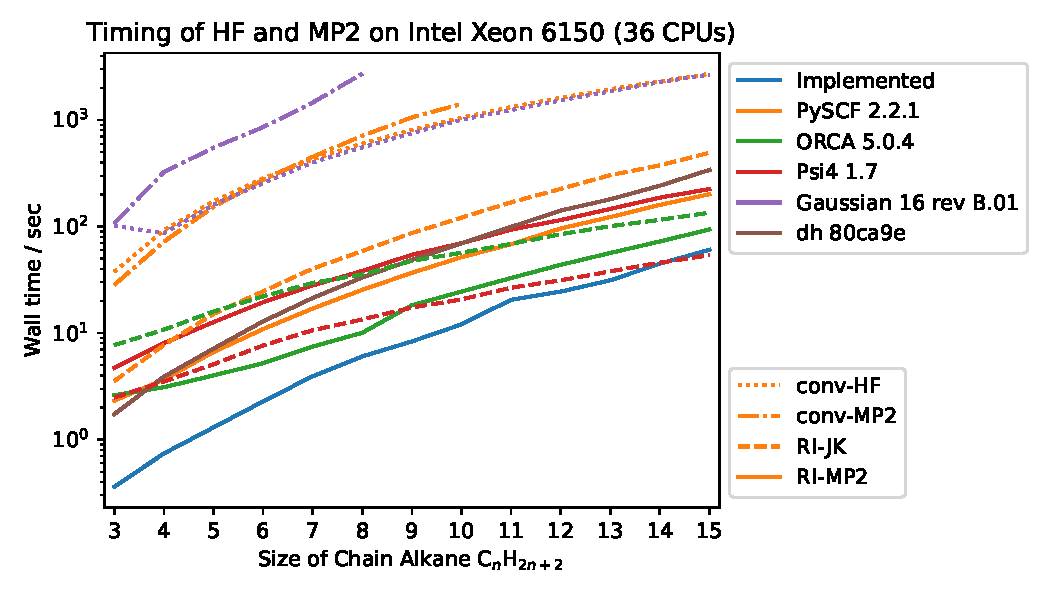
\includegraphics[width=0.8\textwidth]{assets/timing-rimp2-implemented.pdf}

  \raggedright
  \begin{itemize}[nosep]
    \item 测评体系是链状烷烃 \ce{C_n H_{2n+2}},基组 def2-QZVPPD、RI-JK 与 RI-MP2 分别使用对应于 def2-QZVPPD 的辅助基组。计算设备为 Intel Xeon Gold 6150 (36 cores, 72 threads, 2 NUMA nodes);所有计算任务使用 36 线程 (PySCF, Psi4, Gaussian) 或进程 (ORCA) 并行。
    \item 图中 Implemented (蓝色线) 是通过与附录 \ref{sec.python-ri-mp2} 相似的纯 Python 程序的测评结果。
    \item 除 PySCF conv-HF 或 conv-MP2 限制使用 32 GB 内存空间外,其余情形提供 300 GB 的充足内存以保证所有 3c-2e 积分可置于内存中,并使用默认的算法进行计算。
    \item 不同程序的自洽场收敛判据不同、迭代步数不同。3 碳以上所有测评涉及程序的迭代步数一般在 9--11 步。
  \end{itemize}
\end{figure}

\subsubsection{偶极矩与静态极化率:偶极电场下的能量与梯度}

这一小节将引入偶极电场下的梯度量:偶极矩 (dipole) 与静态极化率 (static polarizability)\footnote{需要指出,极化率作为二阶梯度量,与 M\o{}ller-Plesset 二阶微扰 (MP2) 一样,可以通过 Rayleigh-Schr\"odinger 微扰理论导出。在该理论下,还可以得出一定频率下外加偶极电场扰动下能量的变化;此情形下的极化率称为动态极化率 (dynamic polarizability)。动态极化率在以化学增强 SERS 为代表的问题中有重要的意义\cite{Jensen-Schatz.CSR.2008, Perez-Jimenez-Ren.CS.2020, Li-Xu.C.2022};但在本工作中,我们将不考察动态极化率问题。}。

在偶极电场 $\pmb{\mathcal{E}}$ 的微扰下,Hamilton 算符的形式\alert{在绪论中}已经阐明。令外场下微扰 Hamilton 算符为 $\hat H^{(1)}$;微扰算符是由单电子算符与常数项所构成:
\begin{equation}
  \label{eq.electric-perturbed-hamiltonian}
  \hat H^{(1)} = - \sum_i^{n_\mathrm{elec}} \pmb{\mathcal{E}}^\dagger \bm{r}_i + \sum_{A}^{n_\mathrm{atom}} Z_A \pmb{\mathcal{E}}^\dagger \bm{A} \quad \text{(not Einstein notation)}
\end{equation}
作为三维向量的偶极矩 $\bm{\mu}$ 与作为三维矩阵的极化率 $\bm{\alpha}$ 分别定义为分子基态能量受偶极电场扰动的一阶导数与二阶导数量\cite{Atkins-Friedman.Oxford.2011}:
\begin{align}
  E(\pmb{\mathcal{E}}) &= E(\bm{0}) + \pmb{\mathcal{E}}^\dagger \cdot \bm{\mu} - \pmb{\mathcal{E}} \cdot \bm{\alpha} \cdot \pmb{\mathcal{E}} + o(|\pmb{\mathcal{E}}|^3) \notag\\
  &= E(\bm{0}) + \mathcal{E}_t \mu_t - \mathcal{E}_t \alpha_{ts} \mathcal{E}_s + o(|\pmb{\mathcal{E}}|^3)
\end{align}
上式的 $t, s$ 指代坐标分量 $x, y, z$。偶极矩 $\bm{\mu}$ 与极化率 $\bm{\alpha}$ 也可以通过下式定义:
\begin{equation}
  \bm{\mu} := \left. \frac{\mathrm{d} E}{\mathrm{d} \pmb{\mathcal{E}}} \right|_{\pmb{\mathcal{E}} = \bm{0}}, \quad
  \bm{\alpha} := - \left. \frac{\mathrm{d}^2 E}{\mathrm{d} \pmb{\mathcal{E}}^2} \right|_{\pmb{\mathcal{E}} = \bm{0}}
\end{equation}
分量的数值定义为
\begin{equation}
  \mu_t = \left. \frac{\mathrm{d} E}{\mathrm{d} \mathcal{E}_t} \right|_{\pmb{\mathcal{E}} = \bm{0}}, \quad
  \alpha_{ts} = - \left. \frac{\mathrm{d}^2 E}{\mathrm{d} \mathcal{E}_t \mathrm{d} \mathcal{E}_s} \right|_{\pmb{\mathcal{E}} = \bm{0}}
\end{equation}

在计算化学程序中,定义微扰下的单电子积分
\begin{align}
  h_{\mu \nu}^{t} &= - \int \phi_\mu (\bm{r}) t \phi_\nu (\bm{r}) \, \mathrm{d} \bm{r} \\
  \label{eq.def.huv-with-perturb}
  h_{\mu \nu} (\pmb{\mathcal{E}}) &= h_{\mu \nu} (\bm{0}) + \mathcal{E}_t h_{\mu \nu}^t
\end{align}
以及微扰下的原子核能量
\begin{equation}
  E^\textsf{non-elec} (\pmb{\mathcal{E}}) = \frac{1}{2} \frac{Z_A Z_B}{r_{AB}} + Z_A \mathcal{E}_t A_t
\end{equation}
可以求得偶极电场 $\pmb{\mathcal{E}}$ 下的分子能量。因此,偶极矩 $\bm{\mu}$ 与极化率 $\bm{\alpha}$ 可以通过对 $E^\textsf{tot} (\pmb{\mathcal{E}})$ 作数值差分或解析导数得到。

\begin{figure}
  \centering
  \caption{能量在外场下的变化情况 $E(\pmb{\mathcal{E}})$。图中的体系是键长 0.9914 \AA、键角 116.10$^\circ$ 的 \ce{NH_3} 体系;$C_3$ 旋转轴与 $z$ 轴重合;计算模型为 HF/6-31G;外场沿 $z$ 轴即外场强度向量 $\pmb{\mathcal{E}}^\dagger = (0, 0, \mathcal{E}_z)$。蓝色曲线绘制了 $E(\pmb{\mathcal{E}})$ 关于 $\mathcal{E}_z$ 的函数。橙色曲线绘制了 $\mathcal{E}_z = 0$ 时 $\partial_{\mathcal{E}_z} E$ 的导数值;该导数值等于偶极矩在 $z$ 轴上的分量 $\mu_z$。}
  \label{fig.NumDipole-z}
  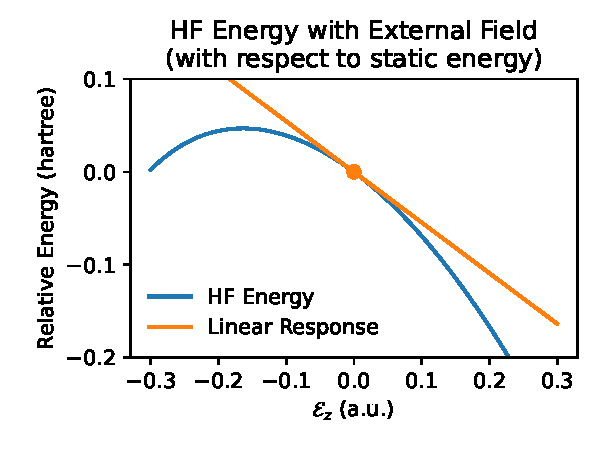
\includegraphics[width=0.5\textwidth]{assets/NumDipole-z.pdf}
\end{figure}

需要指出,式 (\ref{eq.electric-perturbed-hamiltonian}) 所述的 $- \pmb{\mathcal{E}}^\dagger \bm{r}$ 形式的偶极电场仅仅是外加电场其中一种可能性。若外加电场是 $- \pmb{\mathcal{E}}^\dagger \bm{Q} \pmb{\mathcal{E}}$ 的形式,其中
\begin{equation*}
  \bm{Q} =
  \begin{pmatrix}
    x^2 & xy & xz \\
    yx & y^2 & yz \\
    zx & zy & z^2
  \end{pmatrix}
\end{equation*}
那么在该类型的外加电场下,一阶梯度将给出四极矩 (quadrupole)。电场的其它多级展开还将给出八极矩 (octupole)、十六极矩 (hexadecapole) 等等。所有类型的外加电场,在计算化学程序中都表现为对单电子积分与原子核能量的微扰,而对双电子积分、DFA 格点积分能量、原子轨道等部分不产生微扰。本工作着重于极化率,即 $- \pmb{\mathcal{E}}^\dagger \bm{r}$ 形式的偶极电场下的一阶与二阶梯度,即偶极矩与静态极化率的推导与程序实现;但该推导能比较容易地拓展到其它形式的外加电场一阶与二阶梯度。

\subsection{双杂化泛函电性质解析梯度}
\label{sec.3.theory}

本节将在 xDH 框架下,讨论电性质导数问题;被求导的性质将以 $\mathbb{A}, \mathbb{B}$ 表示。除非特别指明,一般讨论的是闭壳层情形。不同于分子坐标导数或 GIAO 轨道导数,许多 Skeleton 导数对于电性质是零值;因此,这里的讨论不适合推广到所有的梯度问题中。

\subsubsection{正交条件、自洽场条件与自洽场泛函对密度矩阵的依赖关系}

在开始梯度理论推演前,先对式 (\ref{eq.def.eng-SCF}) 所给出的自洽场计算过程与结果作必要的回顾。这一小节不考虑外场效应。

作为低阶泛函,闭壳层自洽场能量 $E^\textsf{SCF}$ 仅决定于依式 (\ref{eq.def.dm-scf-closed}) 所定义的双占据的密度矩阵 $D_{\mu \nu}$。密度矩阵 $D_{\mu \nu}$ 由分子轨道系数 $C_{\mu i}$ 构成;分子轨道正交归一条件 (后文简称为\textsf{正交条件}) 具体表达为
\begin{empheq}[box=\fbox]{equation}
  \label{eq.constraint.ortho}
  S_{pq} = C_{\mu p} S_{\mu \nu} C_{\nu q} = \delta_{pq} \quad \text{(orthogonalization constraint)}
\end{empheq}
原子轨道基的 Fock 矩阵定义为自洽场能量对密度矩阵的导数:
\begin{equation}
  \label{eq.def.fock-ao}
  F_{\mu \nu} := \frac{\partial E^\textsf{SCF}}{\partial D_{\mu \nu}}
\end{equation}
它是自洽场作为变分方法的重要中间量,且为对称矩阵。自洽场能量 $E^\textsf{SCF}$ 对占据轨道 $C_{\mu i}$ 的导数为
\begin{align}
  \label{eq.eng-deriv-wrt-coeff}
  \frac{\partial E^\textsf{SCF}}{\partial C_{\mu i}} &= \frac{\partial E^\textsf{SCF}}{\partial D_{\kappa \lambda}} \frac{\partial D_{\kappa \lambda}}{\partial C_{\mu i}}
  = F_{\kappa \lambda} \left( 2 \delta_{\kappa \mu} C_{\lambda i} + 2 \delta_{\lambda \mu} C_{\kappa i} \right) = 4 F_{\mu \nu} C_{\nu i}
\end{align}
占据轨道系数 $C_{\mu i}$ 是通过引入正交条件 (\ref{eq.constraint.ortho}) 对 $E^\textsf{SCF}$ 作条件极小值计算得到。定义对称的 Lagrange 乘子矩阵为 $\varepsilon_{jk}$;下式作为变分方程,对指标 $\nu, j, k$ 求和:
\begin{equation}
  \label{eq.hartree-fock-roothaan}
  \frac{\partial}{\partial C_{\mu i}} \big( E^\textsf{SCF} - 2 \varepsilon_{jk} (S_{jk} - \delta_{jk}) \big) = 4 \big( F_{\mu \nu} C_{\nu i} - S_{\mu \nu} C_{\nu j} \varepsilon_{ji} \big) = 0
\end{equation}
若自洽场泛函是 Hartree-Fock,那么上式即 Hartree-Fock-Roothaan 方程\cite{Roothaan-Roothaan.RMP.1951}。

$F_{\mu \nu}$ 作为原子轨道基下的矩阵,秩 $n_\mathrm{MO}$ 明显大于占据轨道数 $n_\mathrm{nocc}$;在程序实现中,一般将求取 $n_\mathrm{MO}$ 个分子轨道的系数 $C_{\mu p}$:
\begin{equation}
  \label{eq.SCF-working-equation}
  F_{\mu \nu} C_{\nu p} = S_{\mu \nu} C_{\nu q} \varepsilon_{qp} \quad \text{(SCF working equation)}
\end{equation}
但需要注意到,只有占据轨道对自洽场能量产生贡献。关于自洽场对占据布局的限制条件,可以通过对式 (\ref{eq.hartree-fock-roothaan}) 等式两边乘以非占轨道系数 $C_{\mu a}$、并对原子轨道指标 $\mu, \nu$ 求和结果所体现:
\begin{equation*}
  4 (C_{\mu a} F_{\mu \nu} C_{\nu i} - C_{\mu a} S_{\mu \nu} C_{\nu j} \varepsilon_{ji}) = 4 (F_{ai} - S_{aj} \varepsilon_{ji}) = 0
\end{equation*}
或更简洁地,Fock 矩阵在分子轨道基下是分块对角化的:
\begin{empheq}[box=\fbox]{equation}
  \label{eq.constraint.SCF}
  F_{ai} = 0 \quad \text{(SCF constraint)}
\end{empheq}
上式在后文称为\textsf{自洽场条件};推演过程利用了正交条件 (\ref{eq.constraint.ortho}) 所给出的 $S_{aj} = 0$ (占据轨道与非占轨道角标不可能一致)。

正交条件与自洽场条件是梯度推演中,所有必要的额外限制条件。

最后,为了后面推导的便利,这里引入 A 张量的前导张量 $\tilde A_{\mu \nu, \kappa \lambda}$ (Fock 轨道响应张量) 作为 Fock 矩阵对密度矩阵的导数量:
\begin{equation}
  \label{eq.def.Auvkl-pre}
  \tilde A_{\mu \nu, \kappa \lambda} := \frac{\partial^2 E^\textsf{SCF}}{\partial D_{\mu \nu} \partial D_{\kappa \lambda}} = \frac{\partial F_{\mu \nu}}{\partial D_{\kappa \lambda}}
\end{equation}
该张量通常具有 4 重对称性:
\begin{equation*}
  \tilde A_{\mu \nu, \kappa \lambda} = \tilde A_{\kappa \lambda, \mu \nu} = \tilde A_{\nu \mu, \lambda \kappa} = \tilde A_{\lambda \kappa, \nu \mu}
\end{equation*}
但需要指出,若交换能 $E_\mathrm{x}^\textsf{exact}$ (或其长程的对应 $E_\mathrm{x}^\textsf{LR}$) 对能量项有贡献,那么该张量不是 8 重对称性的 (即不满足 $\tilde A_{\mu \nu, \kappa \lambda} = \tilde A_{\mu \nu, \lambda \kappa}$)。出于便利,我们将定义下述 8 重对称性的张量 $A_{\mu \nu, \kappa \lambda}$,该张量称为 A 张量:
\begin{equation}
  \label{eq.def.Auvkl}
  A_{\mu \nu, \kappa \lambda} := 2 \left( \tilde A_{\mu \nu, \kappa \lambda} + \tilde A_{\mu \nu, \lambda \kappa} \right)
\end{equation}
上式定义中的 2 倍,是出于闭壳层情形下,下述表达式方便而给出:
\begin{align}
  \frac{\partial F_{\mu \nu}}{\partial C_{\kappa i}} &= \frac{\partial F_{\mu \nu}}{\partial D_{\eta \lambda}} \frac{\partial D_{\eta \lambda}}{\partial C_{\kappa i}}
  = 2 \tilde A_{\mu \nu, \eta \kappa} \left( \delta_{\eta \kappa} C_{\lambda i} + \delta_{\lambda \kappa} C_{\eta i} \right) \notag\\
  &= 2 \left( \tilde A_{\mu \nu, \kappa \lambda} + \tilde A_{\mu \nu, \lambda \kappa} \right) C_{\lambda i} \notag\\
  &= A_{\mu \nu, \kappa \lambda} C_{\lambda i} = A_{\mu \nu, \kappa i}
\end{align}
上式的第三个等号利用了被求和角标 $\eta, \lambda$ 的轮换。

\subsubsection{一阶梯度:轨道系数随外场的变化}

自洽场泛函 $E^\textsf{SCF}$ 与能量泛函 $E^\textsf{xDH}$ 的运算共用同一轨道系数 $C_{\mu i}$。这一小节进一步讨论正交条件、自洽场条件在外场微扰 $\mathbb{A}$ 下的响应,并籍此给出描述轨道系数在外场微扰下变化的 U 矩阵 $U_{pq}^\mathbb{A}$\footnote{式 (\ref{eq.def.U}) 中 U 矩阵的定义并非在等式左边。利用正交条件 (\ref{eq.constraint.ortho}),可知
\begin{equation*}
  U_{pq}^\mathbb{A} := C_{\mu p} S_{\mu \nu} \partial_\mathbb{A} C_{\nu q}
\end{equation*}
该式与定义式 (\ref{eq.def.U}) 是等价的。出于推演方便,我们仅使用定义式 (\ref{eq.def.U})。}:
\begin{empheq}[box=\fbox]{equation}
  \label{eq.def.U}
  \partial_\mathbb{A} C_{\mu q} = C_{\mu p} U_{pq}^\mathbb{A}
\end{empheq}
这一小节首先确定 U 矩阵在占据-非占部分 $U_{ai}^\mathbb{A}$ 的表达式。其余部分在后一小节详细描述。

对正交条件 (\ref{eq.constraint.ortho}) 作性质 $\mathbb{A}$ 的导数:
\begin{align*}
  \partial_{\mathbb{A}} S_{pq} &= \partial_\mathbb{A} C_{\mu p} S_{\mu \nu} C_{\nu q} + C_{\mu p} \partial_\mathbb{A} S_{\mu \nu} C_{\nu q} + C_{\mu p} S_{\mu \nu} \partial_\mathbb{A} C_{\nu q} \notag\\
  &= S_{mq} U_{mp}^\mathbb{A} + S_{pm} U_{mq}^\mathbb{A} = U_{pq}^\mathbb{A} + U_{qp}^\mathbb{A} = 0
\end{align*}
或更简洁地,
\begin{empheq}[box=\fbox]{equation}
  \label{eq.collary.ortho}
  U_{pq}^\mathbb{A} + U_{qp}^\mathbb{A} = 0 \quad \text{(corollary of orthogonalization constraint)}
\end{empheq}
其中,$\partial_\mathbb{A} S_{pq}$ 推导过程中利用到电性质微扰下基轨道没有变化,因此 $\partial_\mathbb{A} S_{\mu \nu} = 0$。上述结论表明,U 矩阵在电性质导数下是反对称的\footnote{需要指出,对于其它性质梯度,由于 $\partial_\mathbb{A} S_{\mu \nu}$ 未必是零,因此 U 矩阵一般来说未必是反对称或反厄米的。后文将有许多结论只能用于电性质微扰,而无法简单地扩展到所有情形。在本工作中,不会一一列举所有情形。}。

进而将对自洽场条件 (\ref{eq.constraint.SCF}) 的等式两边作性质 $\mathbb{A}$ 的导数。但在考虑 $\partial_\mathbb{A} F_{ai}$ 前,我们先考虑更一般的原子轨道基下 Fock 矩阵的导数:
\begin{equation}
  \label{eq.deduct.pd-Fuv}
  \partial_\mathbb{A} F_{\mu \nu} = \partial_\mathbb{A}^\mathrm{S} F_{\mu \nu} + \partial_\mathbb{A}^\mathrm{U} F_{\mu \nu}
  = F_{\mu \nu}^\mathbb{A} + \frac{\partial F_{\mu \nu}}{\partial C_{\kappa i}} \partial_\mathbb{A} C_{\kappa i}= F_{\mu \nu}^\mathbb{A} + A_{\mu \nu, mi} U_{mi}^\mathbb{A}
\end{equation}
其中,$F_{\mu \nu}^\mathbb{A} := \partial_\mathbb{A}^\mathrm{S} F_{\mu \nu}$ 定义为不受密度矩阵扰动、而仅受外场扰动产生变化的 Skeleton 导数部分。作为特例,对于外加偶极电场而言,从式 (\ref{eq.def.huv-with-perturb}) 附近的讨论出发,仅有单电子算符部分产生贡献:
\begin{align}
  \label{eq.def.sleketon-huv}
  F_{\mu \nu}^{\mathcal{E}_t} = h_{\mu \nu}^{\mathcal{E}_t} &:= \partial_{\mathcal{E}_t} h_{\mu \nu} = h_{\mu \nu}^t \\
  F_{pq}^{\mathcal{E}_t} = h_{pq}^{\mathcal{E}_t} &:= C_{\mu p} F_{\mu \nu}^{\mathcal{E}_t} C_{\nu q}
\end{align}
对于多级展开的外电场也是类似的;我们将在所有电性质导数问题中,假定 $F_{\mu \nu}^\mathbb{A} = h_{\mu \nu}^\mathbb{A}$ 与 $F_{pq}^\mathbb{A} = h_{pq}^\mathbb{A}$。

在得到原子轨道基 Fock 矩阵导数 $\partial_\mathbb{A} F_{\mu \nu}$ 后,分子轨道下的导数可以顺势得到:
\begin{align}
  \label{eq.pd-Fpq-0}
  \partial_\mathbb{A} F_{pq} &= F_{mq} U_{mp}^\mathbb{A} + F_{pm} U_{mq}^\mathbb{A} + C_{\mu p} \partial_\mathbb{A} F_{\mu \nu} C_{\nu q} \notag\\
  &= F_{mq} U_{mp}^\mathbb{A} + F_{pm} U_{mq}^\mathbb{A} + F_{pq}^\mathbb{A} + A_{pq, mj} U_{mj}^\mathbb{A}
\end{align}
上式在二阶梯度求取、以及 MP2 的激发张量导数计算上经常用到;但在这一小节,我们只对其非占-占据部分感兴趣。对自洽场条件 (\ref{eq.constraint.SCF}) 的两边求导,得到
\begin{align}
  \label{eq.pd-Fai-0}
  \partial_\mathbb{A} F_{ai} &= F_{mi} U_{ma}^\mathbb{A} + F_{am} U_{mi}^\mathbb{A} + F_{ai}^\mathbb{A} + A_{ai, mj} U_{mj}^\mathbb{A} = 0
  \quad \text{(corollary of SCF constraint)}
\end{align}
若引入\textsf{正则自洽场条件},即 Fock 矩阵是对角化的:
\begin{equation}
  \label{eq.constraint.canonical-SCF}
  F_{pq} = \varepsilon_p \delta_{pq} \quad \text{(canonical SCF constraint)}
\end{equation}
那么,式 (\ref{eq.pd-Fai-0}) 可以写为
\begin{equation}
  \label{eq.intermediate-pd-Fai-1}
  \partial_\mathbb{A} F_{ai} = \varepsilon_i U_{ia}^\mathbb{A} + \varepsilon_a U_{ai}^\mathbb{A} + F_{ai}^\mathbb{A} + A_{ai, mj} U_{mj}^\mathbb{A} = 0
\end{equation}
该式还可以简化。利用 U 矩阵的反对称性和 A 张量的对称性,$A_{ai, mj} U_{mj}^\mathbb{A}$ 中 $m$ 仅对占据轨道求和时,
\begin{align*}
  \partial_\mathbb{A} F_{ai} \leftarrow A_{ai, kj} U_{kj}^\mathbb{A} = \frac{1}{2} \left( A_{ai, kj} U_{kj}^\mathbb{A} + A_{ai, jk} U_{kj}^\mathbb{A} \right) = \frac{1}{2} \left( A_{ai, kj} U_{kj}^\mathbb{A} + A_{ai, kj} U_{jk}^\mathbb{A} \right) = 0
\end{align*}
上式的 $\leftarrow$ 是指右侧表达式对左侧表达式产生贡献。因此,式 (\ref{eq.intermediate-pd-Fai-1}) 的 $A_{ai, mj} U_{mj}^\mathbb{A}$ 中 $m$ 仅有非占轨道求和的贡献。从而,式 (\ref{eq.intermediate-pd-Fai-1}) 简化为
\begin{empheq}[box=\fbox]{align}
  \label{eq.CP-SCF}
  F_{ai}^\mathbb{A} &= - (\varepsilon_a - \varepsilon_i) U_{ai}^\mathbb{A} - A_{ai, bj} U_{bj}^\mathbb{A} \notag\\
  &= - \left( (\varepsilon_a - \varepsilon_i) \delta_{ai, bj} + A_{ai, bj} \right) U_{bj}^\mathbb{A} \quad \text{(CP-SCF)}
\end{empheq}
该式是电性质导数下的 CP-SCF (\underline{C}oupled-\underline{P}erturbed \underline{SCF}) 方程;通过该方程可以求得 U 矩阵的非占-占据部分 $U_{ai}^\mathbb{A}$。其耦合微扰的意义是,不仅 Hamilton 算符受外场扰动、自洽场波函数也因 Hamilton 算符的微扰而随之产生变化;CP-SCF 方程所给出的 U 矩阵确定了轨道系数 (作为描述自洽场波函数的参数) 是如何随外场发生扰动的。

\subsubsection{一阶梯度:U 矩阵占据-占据和非占-非占部分}
\label{sec.3.Uia-Uai}

对于自洽场方法,轨道正交条件 $S_{pq} = 0$ 与自洽场条件 $F_{ai} = 0$ 是必须满足的条件;但正则自洽场条件 $F_{pq} = \varepsilon_p \delta_{pq}$ 仅仅是出于公式推导的便利与程序实现的方便,而引入的可选条件。这意味着在微扰下,只有占据与非占轨道相互之间的变化情况是非平凡的,即 $U_{ai}^\mathbb{A}$ 与 $U_{ia}^\mathbb{A} = - U_{ai}^\mathbb{A}$ 的数值是非平凡的;占据-占据的 $U_{ij}^\mathbb{A}$ 与非占-非占的 $U_{ab}^\mathbb{A}$ 的数值并非是关键的。因此,只要 $U_{ij}^\mathbb{A}$ 与 $U_{ab}^\mathbb{A}$ 满足式 (\ref{eq.collary.ortho}) 给出的轨道正交条件的结论即可。对于电性质导数而言,最简单的定义方式是置零:
\begin{empheq}[box=\fbox]{equation}
  \label{eq.Uij-Uab-zero}
  U_{ij}^\mathbb{A} = U_{ab}^\mathbb{A} = 0 \quad \text{(definition of program implementation)}
\end{empheq}

在程序实现中,我们将依照式 (\ref{eq.Uij-Uab-zero}) 所给出的定义实现 U 矩阵的占据-占据与非占-非占部分。该式将使得 Fock 矩阵的导数在非对角元上未必为零:
\begin{equation}
  \label{eq.pd-Fpq-not-diagonal}
  \partial_\mathbb{A} F_{pq} \not \equiv 0 \quad (p \neq q, \text{(\ref{eq.Uij-Uab-zero}) satisfied})
\end{equation}
这意味着,Fock 矩阵在外场为零的情形下仍然可以是对角化的,即满足 $F_{pq} |_{\mathbb{A} = 0} = \varepsilon_p \delta_{pq}$;但外场不为零时,Fock 矩阵不再是对角化的;这不同于正交条件与自洽场条件\footnote{许多微扰能形式,譬如 MP2、IEPA、MP2/cr、RPA,在计算时需要引入自洽场轨道能 $\varepsilon_p$;但若 Fock 矩阵 $F_{pq}$ 并非对角的,那么轨道能就无法准确地定义。如果某一方法可以由 Fock 矩阵定义,且无论 Fock 矩阵是否对角、能量结果都是一致的,那么该方法一般来说是正交变换不变的 (Unitary Invariance)。MP2、RPA 方法是正交不变的,但 IEPA、MP2/cr 方法则并非正交不变。这一小节涉及到的推演,特别是式 (\ref{eq.Uij-Uab-zero}) 的定义,应仅对正交不变方法是合理的。}。

下面我们将讨论式 (\ref{eq.pd-Fpq-not-diagonal}) 占据-占据部分情形。利用 Fock 矩阵为对角阵、以及 U 矩阵反对称性质,
\begin{align}
  \partial_\mathbb{A} F_{ij} &= F_{im} U_{mj}^\mathbb{A} + F_{mj} U_{mi}^\mathbb{A} + F_{ij}^\mathbb{A} + A_{ij, mk} U_{mk}^\mathbb{A} \notag\\
  &= (\varepsilon_i - \varepsilon_j) U_{ij}^\mathbb{A} + F_{ij}^\mathbb{A} + A_{ij, bk} U_{bk}^\mathbb{A}
\end{align}
在上式的推导中,当角标 $m$ 作为占据轨道 $l$ 时,贡献项 $\partial_\mathbb{A} F_{ij} \leftarrow A_{ij, lk} U_{lk}^\mathbb{A}$ 由于 $A_{ij, lk}$ 与 $U_{lk}^\mathbb{A}$ 关于 $l, k$ 角标分别对称与反对称,因此该项为零。故而,仅有角标 $m$ 取非占轨道 $b$ 时,$\partial_\mathbb{A} F_{ij} \leftarrow A_{ij, bk} U_{bk}^\mathbb{A}$ 是非平凡的贡献项。通过 CP-SCF 方程,我们已经可以求得 $U_{bj}^\mathbb{A}$;从而,通过上式可以求得
\begin{equation}
  U_{ij}^\mathbb{A} = 
  \begin{cases}
    \displaystyle
    - \frac{F_{ij}^\mathbb{A} + A_{ij, bk} U_{bk}^\mathbb{A} - \partial_\mathbb{A} F_{ij}}{\varepsilon_i - \varepsilon_j} & (i \neq j) \\
    0 & (i = j)
  \end{cases}
\end{equation}
其中,$U_{ii}^\mathbb{A} = 0$ 直接由轨道正交条件 (\ref{eq.collary.ortho}) 所导出。

假使,Fock 矩阵导数也满足正则自洽场条件,即 $\partial_\mathbb{A} F_{ij} = \delta_{ij} \partial_\mathbb{A} \varepsilon_i$,那么
\begin{equation}
  \label{eq.unstable-Uij}
  U_{ij}^\mathbb{A} = - \frac{F_{ij}^\mathbb{A} + A_{ij, bk} U_{bk}^\mathbb{A}}{\varepsilon_i - \varepsilon_j} \quad \left( i \neq j, \, \partial_\mathbb{A} F_{ij} = 0 \right)
\end{equation}
上式的分子一般非零,而分母 $\varepsilon_i - \varepsilon_j$ 则有可能接近于零;举例而言,甲烷分子的最高能级占据轨道为 $T_d$ 不可约表示,即三重简并,因此存在 $i \neq j$ 且 $\varepsilon_i - \varepsilon_j = 0$ 的情形,从而将 $U_{ij}^\mathbb{A}$ 推向无穷大,导致严重的数值误差。因此,为在程序实现中避免这类数值误差,那么 $\partial_\mathbb{A} F_{ij}$ 不适合在 $i \neq j$ 时设为零。

方才分析的是 Fock 矩阵导数占据-占据部分 $\partial_\mathbb{A} F_{ij}$;对于非占-非占部分 $\partial_\mathbb{A} F_{ab}$ 也有类似的结论。

需要指出,尽管令 $\partial_\mathbb{A} F_{pq}$ 为非对角矩阵尽管可以避免数值误差,但同时也有可能增加计算量。对于后续将定义的 MP2 型相关激发张量 $t_{ij}^{ab}$ 的导数,
\begin{equation*}
  \partial_\mathbb{A} t_{ij}^{ab} \leftarrow - \partial_\mathbb{A} F_{ca} t_{ij}^{cb}
\end{equation*}
若 $\partial_\mathbb{A} F_{ca}$ 不是对角矩阵,那么上述贡献项的计算复杂度将是 $O(n_\mathrm{prop} n_\mathrm{occ}^2 n_\mathrm{vir}^3)$,即随体系增大而呈五次复杂度 (作为电性质,偶极外场的 $n_\mathrm{prop} = 3$ 即三个坐标分量方向);但若 $\partial_\mathbb{A} F_{ca}$ 是对角矩阵,则尽管有更低的 $O(n_\mathrm{prop} n_\mathrm{occ}^2 n_\mathrm{vir}^2)$ 即四次复杂度,但仍然是内存密集型运算且存在潜在严重数值误差的可能性。一种可能的解决方案是,对于简并或近简并的一部分轨道,定义非对角的 $\partial_\mathbb{A} F_{pq}$;而剩余下来不存在简并情况的轨道,它们构成的 $\partial_\mathbb{A} F_{pq}$ 仍然是对角的。在这种方案下由于三维空间的最大不可约表示是三维,因此 FLOPs 不会超过 9 倍于 $n_\mathrm{prop} n_\mathrm{occ}^2 n_\mathrm{vir}^2$ 的乘积累加运算\cite{Stoychev-Neese.JCTC.2018}。但这种方案并非简单的张量乘积,程序实现上会引入一定的复杂性;在我们目前的程序实现中,没有将其纳入考虑。

\subsubsection{一阶梯度:能量泛函导数}

这一小节讨论能量泛函 $E^\textsf{xDH}$ 在性质 $\mathbb{A}$ 微扰下的导数。

xDH 总能量的全导数可以分为 Skeleton 部分与对轨道系数的导数两部分:
\begin{equation}
  \label{eq.def.pdA-xDH-0}
  \partial_\mathbb{A} E^\textsf{xDH} = \partial_\mathbb{A}^\mathrm{S} E^\textsf{xDH} + \frac{\partial E^\textsf{xDH}}{\partial C_{\mu q}} \partial_\mathbb{A} C_{\mu q}
\end{equation}
对于轨道系数导数部分,我们作更多讨论。定义 xDH 的广义 Fock 矩阵 (generalized Fock matrix) 为
\begin{equation}
  \label{eq.def.generalized-fock}
  F_{pq}^\textsf{xDH} := C_{\mu p} \frac{\partial E^\textsf{xDH}}{\partial C_{\mu q}}
\end{equation}
该矩阵的性质是
\begin{itemize}[nosep]
  \item 若 $E^\textsf{xDH} = E^\textsf{SCF}$,则广义 Fock 矩阵的占据-占据部分 $F_{ij}^\textsf{xDH}$ 退化到自洽场 Fock 矩阵 $F_{ij}$;但非占-非占部分 $F_{ab}^\textsf{xDH}$ 数值上是零,因非占轨道对自洽场能量没有影响;
  \item 广义 Fock 矩阵不一定是对角化的、对称的;非占-占据或占据-非占部分也未必为零\footnote{对于一般的 bDH 或 xDH 型泛函,广义 Fock 矩阵不一定对角化。轨道优化 (orbital-optimized) MP2 或双杂化泛函,则要求广义 Fock 矩阵对角化是对角化的\cite{Bozkaya-Sherrill.JCP.2011}。但轨道优化的代价,是要多次迭代地计算广义 Fock 矩阵、单步 MP2 相关能因非正则 SCF 的缘故需迭代计算得到,且广义 Fock 矩阵计算消耗一般不小于 MP2 相关能计算。}。
\end{itemize}
进而引入 xDH Lagrangian 为广义 Fock 反对称化矩阵\footnote{在本文中,Lagrangian 通过广义 Fock 矩阵所定义。但一般来说,Lagrangian 应当通过轨道或密度在旋转矩阵下的导数定义\cite{Helgaker-Jorgensen.Wiley.2013};因此,应当认为广义 Fock 反对称化矩阵的结果等于 Lagrangian,而非后者为前者所定义。但比较严格地引入 Lagrangian 将占用一定的篇幅。}:
\begin{equation}
  \label{eq.def.lagrangian}
  L_{pq}^\textsf{xDH} := F_{pq}^\textsf{xDH} - F_{qp}^\textsf{xDH}
\end{equation}
注意到对于电性质而言,U 矩阵是反对称、且在占据-占据部分与非占-非占部分可以置零;因此,
\begin{align}
  \label{eq.derivation-contrib-Lai-to-engderiv}
  \partial_\mathbb{A} E^\textsf{xDH} &\leftarrow \frac{\partial E^\textsf{xDH}}{\partial C_{\mu q}} \frac{\partial C_{\mu q}}{\partial \mathbb{A}} = F_{pq}^\textsf{xDH} U_{pq}^\mathbb{A} \notag\\
  &= F_{ai}^\textsf{xDH} U_{ai}^\mathbb{A} + F_{ia}^\textsf{xDH} U_{ia}^\mathbb{A} + F_{ij}^\textsf{xDH} U_{ij}^\mathbb{A} + F_{ab}^\textsf{xDH} U_{ab}^\mathbb{A} \notag\\
  &= (F_{ai}^\textsf{xDH} - F_{ia}^\textsf{xDH}) U_{ai}^\mathbb{A} + 0 = L_{ai}^\textsf{xDH} U_{ai}^\mathbb{A}
\end{align}
特别地,对于自洽场方法,$L_{ai}^\textsf{SCF} = 0$。从而,电性质微扰下 xDH 一阶泛函能量导数可以写为
\begin{empheq}[box=\fbox]{equation}
  \label{eq.derivation-xdh-energy-deriv-abstract}
  \partial_\mathbb{A} E^\textsf{xDH} = \partial_\mathbb{A}^\mathrm{S} E^\textsf{xDH} + L_{ai}^\textsf{xDH} U_{ai}^\mathbb{A}
\end{empheq}

正因为 xDH 型泛函包含了公式形式复杂的 $E^\textsf{PT} [\mathbf{C}]$、以及其 Lagrangian 一般地非零 $L_{ai}^\textsf{xDH} \not \equiv 0$,从而 xDH 型泛函的梯度理论相比之自洽场而言要复杂不少。

\subsubsection{一阶梯度:约化密度矩阵}

约化密度与电性质 Skeleton 导数有直接的联系。这里先以 CI 波函数 $| \Psi^\textsf{CI} \rangle$ 开始讨论,随后引申到 xDH 型泛函的约化密度。本小节与下一小节同时参考 Trucks 等的文献\cite{Trucks-Bartlett.CPL.1988}。

CI 的 (一阶) 约化密度 (RDM, \underline{R}educed \underline{D}ensity \underline{M}atrix) 在分子轨道基下,一般定义为
\begin{equation}
  \label{eq.def.rdm-ci}
  D_{qp}^{\textsf{CI},\textsf{RDM}} := \frac{\langle \Psi^\textsf{CI} | a_p^\dagger a_q | \Psi^\textsf{CI} \rangle}{\langle \Psi^\textsf{CI} | \Psi^\textsf{CI} \rangle}
\end{equation}
约化密度矩阵的意义是,对于任意的单电子算符 $\hat o = o_{pq} a_p^\dagger a_q$,其期望值总是可以写为约化密度矩阵 $D_{qp}^{\textsf{CI},\textsf{RDM}}$ 与算符矩阵表示 $o_{pq}$ 的乘积:
\begin{equation*}
  \langle \hat o \rangle = \frac{\langle \Psi^\textsf{CI} | \hat o | \Psi^\textsf{CI} \rangle}{\langle \Psi^\textsf{CI} | \Psi^\textsf{CI} \rangle} = o_{pq} D_{qp}^{\textsf{CI},\textsf{RDM}}
\end{equation*}
注意到 $(a_p^\dagger a_q)^\dagger = a_q^\dagger a_p$,因此 $D_{qp}^{\textsf{CI},\textsf{RDM}}$ 是复共轭的。由于本工作仅考虑实数范围内的问题,因此可以认为约化密度矩阵是对称的。

现在考虑 CI 波函数的电性质 Skeleton 导数问题。对于 Hamilton 算符 $\hat H$,电子所引起的能量效应中,电性质仅对单电子算符 $\hat h = \hat T + \hat V_\mathrm{ext}$ 中的外势 $\hat V_\mathrm{ext}$ 有微扰贡献:
\begin{equation}
  \partial_\mathbb{A}^\mathrm{S} \hat H = \partial_\mathbb{A}^\mathrm{S} \hat h + \partial_\mathbb{A} \hat V_\textsf{non-elec} = h_{pq}^\mathbb{A} a_p^\dagger a_q + \partial_\mathbb{A} \hat V_\textsf{non-elec}
\end{equation}
依 Hellmann-Feynman 定理,算符期望的 Skeleton 导数等于 Skeleton 导数下算符的期望:
\begin{equation}
  \partial_\mathbb{A}^\mathrm{S} E^\textsf{CI} = \partial_\mathbb{A}^\mathrm{S} \langle \hat H \rangle = \langle \partial_\mathbb{A}^\mathrm{S} \hat H \rangle = \langle \partial_\mathbb{A}^\mathrm{S} \hat h \rangle + \partial_\mathbb{A} E^\textsf{non-elec} = h_{pq}^\mathbb{A} D_{pq}^{\textsf{CI}, \textsf{RDM}} + \partial_\mathbb{A} E^\textsf{non-elec}
\end{equation}

但作为常见的 xDH 型泛函能量贡献项,MP2 相关能或其它形式的相关能,在定义约化密度的问题上存在一些困难。MP2 方法的波函数并非是对 $\hat H$ 变分极小的,因此 Hellmann-Feynman 定理失效,从而 MP2 方法的约化密度矩阵不能通过与 CI 相同的方式 (\ref{eq.def.rdm-ci}) 所定义\footnote{
  注意到 MP2 相关能可以通过 Hylleraas 泛函给出\cite{Hylleraas-Hylleraas.ZP.1930, Pulay-Saeboe.TCA.1986}:
  \begin{equation*}
    E_\mathrm{c}^\textsf{(2)} = \min_{\Psi^{(1)}} \left( 2 \langle \Psi^\textsf{(1)} | \hat H - E^\textsf{0} | \Phi^\textsf{0} \rangle - \langle \Psi^\textsf{(1)} | \hat F - E^\textsf{0} | \Psi^\textsf{(1)} \rangle \right)
  \end{equation*}
  这里的 $\Phi^\textsf{0}$ 是 Hartree-Fock 行列式,$E^\textsf{0} = \langle \Phi^\textsf{0} | \hat F | \Phi^\textsf{0} \rangle$ 为零阶能量 (占据轨道能之和),$\Psi^\textsf{(1)}$ 是 MP2 相关波函数。上式可以看作对 $\Psi^\textsf{(1)}$ 取变分极小,因此 Hellmann-Feynman 定理适用于此。又由于 Brillouin 定理,$\Psi^\textsf{(1)}$ 只有二次激发项贡献、没有单次激发项,故对于任何单电子算符 $\hat o$ 总有 $\langle \Psi^\textsf{(1)} | \hat o | \Phi^\textsf{0} \rangle = 0$。故 MP2 相关部分对约化密度矩阵贡献是
  \begin{equation*}
    D_{pq}^{\textsf{(2)},\textsf{RDM}} = - \langle \Psi^\textsf{(1)} | a_p^\dagger a_q | \Psi^\textsf{(1)} \rangle
  \end{equation*}
  上述推导是基于自旋轨道下的;应当可以验证,在开壳层或闭壳层的限制下,通过 $\partial_\mathbb{A}^\mathrm{S} E \leftarrow h_{pq}^\mathbb{A} D_{pq}^\textsf{RDM}$ 给出的约化密度矩阵,与通过二次量子化算符下给出的约化密度矩阵是一致的。
}。但我们注意到,若能量的电性质 Skeleton 导数的电子效应部分可以写为下述矩阵乘积与非电子效应导数之和:
\begin{empheq}[box=\fbox]{equation}
  \label{eq.collary.rdm-definition}
  \partial_\mathbb{A}^\mathrm{S} E = h_{pq}^\mathbb{A} D_{pq}^\textsf{RDM} + \partial_\mathbb{A} E^\textsf{non-elec} \quad \text{(electric property)}
\end{empheq}
那么就可以从 Skeleton 导数 $\partial_\mathbb{A}^\mathrm{S} E$ 推出约化密度矩阵 $D_{pq}^\textsf{RDM}$\footnote{
  但注意到,若是其它性质,譬如原子核导数问题,Skeleton 导数对基组本身产生扰动,因而式 (\ref{eq.def-E-tot}) 所定义的能量项的每一项都有 Skeleton 导数的贡献;这将导致表达式较为复杂,即单电子 Skeleton 导数 $\partial_\mathbb{A}^\mathrm{S} E \leftarrow h_{pq}^\mathbb{A} D_{pq}^\textsf{RDM}$ 只是原子核导数问题的其中一个电子效应贡献项。因此,通过 Skeleton 导数给出约化密度,只能在电性质梯度下、或其它仅对单电子算符产生微扰的性质下,方能成立。
}。该约化密度矩阵的定义不仅适用于 MP2 等非变分的后自洽场方法,也适用于 xDH 型泛函。我们记 xDH 型泛函的约化密度为 $D_{pq}^{\textsf{xDH}, \textsf{RDM}}$。

\subsubsection{一阶梯度:Z-Vector 方法与弛豫密度}

式 (\ref{eq.derivation-xdh-energy-deriv-abstract}) 中 $\partial_\mathbb{A} E^\textsf{xDH}$ 求取的第二项可以进一步整理。该整理过程对二阶梯度的推导也是重要的。

注意到 $U_{ai}^\mathbb{A}$ 有三个角标,其张量维度是 $(n_\mathrm{prop}, n_\mathrm{vir}, n_\mathrm{occ})$。$U_{ai}^\mathbb{A}$ 的求取是通过 CP-SCF 方程 (\ref{eq.CP-SCF}) 给出,其计算量在不预先存储 A 张量 $A_{ia, jb}$ 时较大,是有效率优化价值的计算过程。

Handy 与 Schaefer III 指出\cite{Handy-Schaefer.JCP.1984},对于一阶梯度,若 Lagrangian 为 $L_{ai}$,则不需要求取 $(n_\mathrm{prop}, n_\mathrm{vir}, n_\mathrm{occ})$ 维度的 U 矩阵 $U_{ai}^\mathbb{A}$,而只需要求取 $(n_\mathrm{vir}, n_\mathrm{occ})$ 维度的 Z 矩阵 $Z_{ai}$:
\begin{empheq}[box=\fbox]{equation}
  \label{eq.Z-vector}
  - (\varepsilon_a - \varepsilon_i) Z_{ai} - A_{ai, bj} Z_{bj} = L_{ai} \quad \text{(definition of } Z_{ai} \text{)}
\end{empheq}
在本工作中,该方程称为 Z-Vector 方程。那么 Lagrangian 对能量的贡献可以化为
\begin{empheq}[box=\fbox]{equation}
  \label{eq.Z-vector-contrib-to-eng-deriv}
  \partial_\mathbb{A} E \leftarrow L_{ai} U_{ai}^\mathbb{A} = Z_{ai} F_{ai}^\mathbb{A}
\end{empheq}

这里有必要回顾 Z-Vector 方法,因为其推演过程将对二阶梯度的计算有所帮助。为方便起见,定义
\begin{equation}
  \label{eq.def.scrA}
  \mathscr{A}_{ai,bj} := - \left( (\varepsilon_a - \varepsilon_i) \delta_{ai, bj} + A_{ai, bj} \right)
\end{equation}
现在将角标 $ai$ 和 $bj$ 看作联合角标 (即将 $Z_{ai}$ 视作关于角标 $ai$ 的一维向量 $\mathbf{Z}$、将 $\mathscr{A}_{ai, bj}$ 视作关于角标 $ai$、$bj$ 的二维矩阵 $\pmb{\mathscr{A}}$)。那么,CP-SCF 方程 (\ref{eq.CP-SCF}) 与 Z-Vector 方程 (\ref{eq.Z-vector}) 分别写为
\begin{align}
  \label{eq.CP-SCF-matrix-form}
  \pmb{\mathscr{A}} \mathbf{U}^\mathbb{A} &= \mathbf{F}^\mathbb{A} \\
  \label{eq.Z-Vector-matrix-form}
  \pmb{\mathscr{A}} \mathbf{Z} &= \mathbf{L}
\end{align}
从而,U 矩阵可以表示为 $\mathbf{U}^\mathbb{A} = \pmb{\mathscr{A}}^{-1} \mathbf{F}^\mathbb{A}$,Z 矩阵可以表示为 $\mathbf{Z} = \pmb{\mathscr{A}}^{-1} \mathbf{L}$。注意到 $\mathscr{A}_{ai,bj} = \mathscr{A}_{bj,ai}$ 即 $\pmb{\mathscr{A}}$ 具有对称性,式 (\ref{eq.derivation-xdh-energy-deriv-abstract}) 中 Lagrangian 对能量的贡献,可以写为
\begin{equation}
  \partial_\mathbb{A} E \leftarrow \mathbf{L}^\dagger \mathbf{U}^\mathbb{A} = \mathbf{L}^\dagger (\pmb{\mathscr{A}}^{-1} \mathbf{F}^\mathbb{A}) = \mathbf{L}^\dagger (\pmb{\mathscr{A}}^{-1} \mathbf{F}^\mathbb{A}) = (\pmb{\mathscr{A}}^{-1} \mathbf{L})^\dagger \mathbf{F}^\mathbb{A} = \mathbf{Z}^\dagger \mathbf{F}^\mathbb{A}
\end{equation}
这就证明了式 (\ref{eq.Z-vector-contrib-to-eng-deriv})。该推导也适用于 xDH 型泛函;我们记 xDH 型泛函的 Z 矩阵为 $Z_{ai}^\textsf{xDH}$。

最后,我们引入弛豫密度矩阵 (Response/Relax/Lagragian Density Matrix)。注意到对于 xDH 型泛函,由式 (\ref{eq.collary.rdm-definition}) 给出的电性质的 Skeleton 导数对总梯度的贡献是 $\partial_\mathbb{A} E^\textsf{xDH} \leftarrow \partial_\mathbb{A}^\mathrm{S} E^\textsf{xDH} = D_{pq}^{\textsf{xDH}, \textsf{RDM}} F_{pq}^\mathbb{A} + \partial_\mathbb{A} E^\textsf{non-elec}$,轨道导数对总梯度的贡献是 $\partial_\mathbb{A} E^\textsf{xDH} \leftarrow L_{ai}^\textsf{xDH} U_{ai}^\mathbb{A} = Z_{ai}^\textsf{xDH} F_{ai}^\mathbb{A}$;两者都可以写为矩阵与 $F_{pq}^\mathbb{A}$ 的乘积之和。那么就令 xDH 弛豫密度 $D_{pq}^\textsf{xDH}$ 为 xDH 约化密度与 Z 矩阵之和;弛豫密度与 Fock 矩阵 Skeleton 导数的乘积和就是 xDH 型泛函电子效应的电性质梯度:
\begin{empheq}[box=\fbox]{align}
  \label{eq.def.xdh-resp-dm}
  D_{pq}^\textsf{xDH} &:= D_{pq}^{\textsf{xDH}, \textsf{RDM}} + Z_{ai}^{\textsf{xDH}} \delta_{ap} \delta_{qi} \\
  \label{eq.collary.deriv-xdh-1st-order}
  \partial_\mathbb{A} E^\textsf{xDH} &= D_{pq}^\textsf{xDH} F_{pq}^\mathbb{A} + \partial_\mathbb{A} E^\textsf{non-elec}
\end{empheq}

\subsubsection{二阶梯度:二阶能量泛函导数}

从式 (\ref{eq.collary.deriv-xdh-1st-order}),利用链式法则,立即可以导出 xDH 能量泛函的电性质二阶导数:
\begin{empheq}[box=\fbox]{equation}
  \label{eq.def.second-deriv-xdh-eng}
  \partial_\mathbb{A} \partial_\mathbb{B} E^\textsf{xDH} = D_{pq}^\textsf{xDH} \partial_\mathbb{B} F_{pq}^\mathbb{A} + \partial_\mathbb{B} D_{pq}^{\textsf{xDH}, \textsf{RDM}} F_{pq}^\mathbb{A} + \partial_\mathbb{B} Z_{ai}^\textsf{xDH} F_{ai}^\mathbb{A} + \partial_\mathbb{A} \partial_\mathbb{B} E^\textsf{non-elec}
\end{empheq}

式 (\ref{eq.def.second-deriv-xdh-eng}) 的第一项比较容易求取:
\begin{equation}
  \label{eq.second-deriv-xdh-eng-term1}
  \partial_\mathbb{B} F_{pq}^\mathbb{A} = U_{mp}^\mathbb{B} F_{mq}^\mathbb{A} + U_{mq}^\mathbb{B} F_{mp}^\mathbb{A} + F_{pq}^\mathbb{AB}
\end{equation}
特别地,对于外加偶极电场而言,由于式 (\ref{eq.def.huv-with-perturb}) 所给出的 $h_{\mu\nu} (\pmb{\mathcal{E}})$ 关于外场 $\pmb{\mathcal{E}}$ 的微扰只有一阶项,因此二阶导数为零即当 $\mathbb{A}, \mathbb{B}$ 指代电场微扰量 $\pmb{\mathcal{E}}$ 时,$F_{pq}^\mathbb{AB} = 0$。非电子效应项出于同样的理由,也有 $\partial_\mathbb{A} \partial_\mathbb{B} E^\textsf{non-elec} = 0$。

式 (\ref{eq.def.second-deriv-xdh-eng}) 的第二项需要求取 xDH 的约化密度梯度;对于不同的泛函而言,其具体表达式不同,我们将在后一节中对 MP2 型 xDH 泛函的具体实现作更多说明。

\subsubsection{二阶梯度:Z 矩阵导数与交换定理}

式 (\ref{eq.def.second-deriv-xdh-eng}) 的第三项需要求取 Z 矩阵的导数与 Fock 矩阵 Skeleton 导数的乘积和。这里我们将用与 Z-Vector 方法相同的思路处理该项的计算。

首先回顾到一阶梯度的运算。从式 (\ref{eq.collary.deriv-xdh-1st-order}) 的推导结果与式 (\ref{eq.Z-vector}) 附近的讨论来看,xDH 能量的一阶梯度不需要给出 $(n_\mathrm{prop}, n_\mathrm{vir}, n_\mathrm{occ})$ 维度的 U 矩阵 $U_{ai}^\mathbb{A}$,而只需要计算出 $(n_\mathrm{vir}, n_\mathrm{occ})$ 维度的 Z 矩阵 $Z_{ai}$;这很大程度上是为了节省计算量。但对于二阶梯度,对式 (\ref{eq.second-deriv-xdh-eng-term1}) 的计算不可避免地用到 U 矩阵。因此,这里的推导以已经计算得到 U 矩阵为前提。

首先仿照式 (\ref{eq.Z-vector-contrib-to-eng-deriv}) 的形式,写出 Z 矩阵导数对能量二阶梯度的贡献:
\begin{equation}
  \partial_\mathbb{A} \partial_\mathbb{B} E \leftarrow \partial_\mathbb{B} \mathbf{Z}^\dagger \mathbf{F}^\mathbb{A}
\end{equation}
为给出 Z 矩阵的导数 $\partial_\mathbb{B} Z_{ai}$,我们对式 (\ref{eq.Z-Vector-matrix-form}) 两边作关于性质 $\mathbb{B}$ 的导数:
\begin{equation*}
  \partial_\mathbb{B} \pmb{\mathscr{A}} \mathbf{Z} + \pmb{\mathscr{A}} \partial_\mathbb{B} \mathbf{Z} = \partial_\mathbb{B} \mathbf{L}
\end{equation*}
定义
\begin{equation*}
  \pmb{\mathscr{R}}^\mathbb{B} = \partial_\mathbb{B} \mathbf{L} - \partial_\mathbb{B} \pmb{\mathscr{A}} \mathbf{Z}
\end{equation*}
或依矩阵元素的定义
\begin{equation}
  \label{eq.def.Rai-B}
  \mathscr{R}_{ai}^\mathbb{B} := \partial_\mathbb{B} L_{ai} - \partial_\mathbb{B} \mathscr{A}_{ai, bj} Z_{bj}
\end{equation}
于是可整理得到
\begin{equation}
  \pmb{\mathscr{A}} \partial_\mathbb{B} \mathbf{Z} = \pmb{\mathscr{R}}^\mathbb{B}
\end{equation}
这意味着求取维度为 $(n_\mathrm{prop}, n_\mathrm{vir}, n_\mathrm{occ})$ 的 $\partial_\mathbb{B} Z_{ai}$ 矩阵导数,需要与 CP-SCF 相同的计算过程。但事实上,可以再一次使用 Z-Vector 方法避免直接求取 $\partial_\mathbb{B} Z_{ai}$。利用式 (\ref{eq.CP-SCF-matrix-form}) 的结论,
\begin{equation*}
  \partial_\mathbb{A} \partial_\mathbb{B} E \leftarrow \partial_\mathbb{B} \mathbf{Z}^\dagger \mathbf{F}^\mathbb{A} = (\pmb{\mathscr{A}}^{-1} \pmb{\mathscr{R}}^\mathbb{B})^\dagger \mathbf{F}^\mathbb{A} = \pmb{\mathscr{R}}^\mathbb{B}{}^\dagger (\pmb{\mathscr{A}}^{-1} \mathbf{F}^\mathbb{A}) = \pmb{\mathscr{R}}^\mathbb{B}{}^\dagger \mathbf{U}^\mathbb{A}
\end{equation*}
或者写为矩阵元素乘积和的形式:
\begin{empheq}[box=\fbox]{equation}
  \label{eq.interchange-theorem}
  \partial_\mathbb{A} \partial_\mathbb{B} E \leftarrow \mathscr{R}_{ai}^\mathbb{B} U_{ai}^\mathbb{A}
\end{empheq}
该过程也被称为交换定理 (interchange theorem)\cite{Cammi-Frisch.TCA.2004}。

Z 矩阵导数对总能量二阶梯度的贡献,其求取难度在于如何给出 $\partial_\mathbb{B} L_{ai}$ 与 $\partial_\mathbb{B} \mathscr{A}_{ai, bj}$。其中,式 $\partial_\mathbb{B} \mathscr{A}_{ai, bj}$ 在这里可以进一步展开讨论。注意到式 (\ref{eq.def.scrA}) 对 $\mathscr{A}_{ai, bj}$ 的定义中,存在轨道能 $\varepsilon_p$;但在 \ref{sec.3.Uia-Uai} 小节中的讨论中,表明由于轨道能的导数本身只在正则自洽场条件下成立、而这将会使得 U 矩阵的占据-占据与非占-非占部分 $U_{ij}^\mathbb{A}, U_{ab}^\mathbb{A}$ 出现数值问题。由于二阶梯度 (\ref{eq.def.second-deriv-xdh-eng}) 的其它项计算中确实需要使用到 $U_{ij}^\mathbb{A}, U_{ab}^\mathbb{A}$,因而我们不能简单地对轨道能导数 $\partial_\mathbb{B} \varepsilon_p$ 直接作计算。为此,我们回顾式 (\ref{eq.pd-Fai-0}),并注意到自洽场条件 (\ref{eq.constraint.SCF}) 与 U 矩阵反对称性 (\ref{eq.collary.ortho}),在允许非正则 SCF 的情形下对 $\mathscr{A}_{ai, bj}$ 作重新定义:
\begin{equation}
  \label{eq.def.scrA-noncanonical}
  \mathscr{A}_{ai, bj} := F_{ij} \delta_{ab} - F_{ab} \delta_{ij} - A_{ai, bj}
\end{equation}
其全导数的项目很多,但都可以利用基本的链式法则给出。

\subsubsection{总结}

至此,我们推演了 xDH 框架下双杂化泛函的电性质一阶与二阶梯度。目前为止的推演没有引入具体的能量计算表达式,因此该推导预期应可用于任何基于 SCF 所给出的分子轨道 $C_{\mu p}$、进行非变分能量 $E^\textsf{xDH}$ 计算的方法;这种计算方法可以是类如 B2PLYP 的能量泛函中低阶部分与自洽场相同的 bDH 泛函、可以是类如 XYGJ-OS 的 OS-MP2 型泛函、也应预期可以是 dRPA75 的 RPA 型泛函。为具体地实现该框架下的二阶梯度程序化,需要做的是细化框架的表达式。

这里总结二阶梯度的计算流程,以及有必要进行细化的表达式:
\begin{itemize}[nosep]
  \item 电性质的梯度量 $F_{\mu \nu}^\mathbb{A} = h_{\mu \nu}^\mathbb{A}$,对于偶极外场依式 (\ref{eq.def.sleketon-huv}) 给出;
  \item 自洽场泛函 A 张量 $A_{\mu \nu, \kappa \lambda}$ 依式 (\ref{eq.def.Auvkl}) 给出;该项有待细化;
  \item 能量泛函的广义 Fock 矩阵 $F_{pq}^\textsf{xDH}$ 与 Lagrangian $L_{ai}^\textsf{xDH}$ 分别依式 (\ref{eq.def.generalized-fock}, \ref{eq.def.lagrangian}) 给出;该项有待细化;
  \item 通过 Z-Vector 方法,通过与 CP-SCF 相同的计算过程 (\ref{eq.Z-vector}) 给出 Z 矩阵 $Z_{ai}^\textsf{xDH}$;
  \item 通过类如式 (\ref{eq.def.rdm-ci}) 所使用的二次量子化算符运算、或通过式 (\ref{eq.collary.rdm-definition}) 的 Skeleton 导数推演,给出能量泛函对应的约化密度矩阵 $D_{pq}^{\textsf{xDH}, \textsf{RDM}}$,进而依式 (\ref{eq.def.xdh-resp-dm}) 与 Z 矩阵结合给出弛豫密度 $D_{pq}^\textsf{xDH}$;该项有待细化;
  \item 通过式 (\ref{eq.collary.deriv-xdh-1st-order}) 给出能量一阶梯度$\partial_\mathbb{A} E^\textsf{xDH}$;
  \item 描述轨道旋转的 U 矩阵的非占-占据部分 $U_{ai}^\mathbb{A}$ 依式 (\ref{eq.CP-SCF}) 给出;占据-非占部分 $U_{ia}^\mathbb{A}$ 依轨道正交条件推论 (\ref{eq.collary.ortho}) 给出;其余部分对于电性质可以依式 (\ref{eq.Uij-Uab-zero}) 直接置零,也可以依其它规则给出;
  \item 电性质的二阶梯度量 $F_{\mu \nu}^\mathbb{AB}$,对于偶极外场为零;
  \item 依导数规则求取 Fock 导数 $\partial_\mathbb{B} F_{pq}$、约化密度导数 $\partial_\mathbb{B} D_{pq}^{\textsf{xDH}, \textsf{RDM}}$、Lagrangian 导数 $\partial_\mathbb{B} L_{ai}$、A 张量导数 $\partial_\mathbb{B} A_{ai, bj}$,计算得到 $\mathscr{R}_{ai}^\mathbb{B}$ (\ref{eq.def.Rai-B}) 并最终汇总到能量二阶梯度 $\partial_\mathbb{A} \partial_\mathbb{B} E^\textsf{xDH}$ (\ref{eq.def.second-deriv-xdh-eng})。
\end{itemize}

\subsection{闭壳层 MP2 型双杂化泛函解析静态极化率程序化}
\label{sec.3.program}

\subsubsection{记号定义与补充说明}

这一节中,我们将具体地考察双杂化泛函在偶极电场下的二阶梯度计算过程与程序化思路。关于程序化实现的一些具体路线与限制、以及必要的补充记号定义是
\begin{itemize}[nosep]
  \item 可以实现以 XYG7 (作为区分同自旋与异自旋 MP2 相关能的泛函)、$\omega$B97X-2(TQZ) (作为含有长程交换能的泛函)、TPSS0-DH (作为含有 meta-GGA 的双杂化泛函)、lrc-XYG3 (作为含有普通、长程、短程 MP2 相关能的泛函) 等为代表的双杂化泛函的极化率计算。
  \item 对于含有多种 MP2 相关能形式的泛函 (以 lrc-XYG3、RS-PBE-P86 为代表),其微扰能形式是
        \begin{equation*}
          E^\textsf{PT} = c_\mathrm{c}^\textsf{(2)} E_\mathrm{c}^\textsf{(2)} + c_\mathrm{c}^{\textsf{(2)}, \textsf{LR}} E_\mathrm{c}^{\textsf{(2)}, \textsf{LR}} + c_\mathrm{c}^{\textsf{(2)}, \textsf{SR}} E_\mathrm{c}^{\textsf{(2)}, \textsf{SR}}
        \end{equation*}
        假使我们希望求取微扰能对 Lagrangian 的贡献,那么这类泛函的贡献应写为
        \begin{equation*}
          L_{ai}^\textsf{PT} = c_\mathrm{c}^\textsf{(2)} L_{ai}^\textsf{(2)} + c_\mathrm{c}^{\textsf{(2)}, \textsf{LR}} L_{ai}^{\textsf{(2)}, \textsf{LR}} + c_\mathrm{c}^{\textsf{(2)}, \textsf{SR}} L_{ai}^{\textsf{(2)}, \textsf{SR}}
        \end{equation*}
        即微扰总 Lagrangian 的贡献等于各子项的 Lagrangian、依其对能量贡献的比例的加权和。这种可加性也同样可以应用到交换相关泛函的子项拆分;以及弛豫密度、Z 矩阵、A 张量等也适用这种可加性。同时,除了使用了不同类型但维度相同的 ERI,短程、长程 MP2 相关能计算方式与普通的 MP2 完全一致;因此,不失一般性,我们仅讨论 $E^\textsf{PT} = c_\mathrm{c}^\textsf{(2)} E_\mathrm{c}^\textsf{(2)}$ 的情形,而在程序中实现所有类型的 MP2 相关能。
  \item 对于含有多种严格交换能的泛函 (以 $\omega$B97X-2(TQZ)、RS-PBE-P86 为代表),首先短程交换能 $E_\mathrm{x}^\textsf{SR}$ 可以拆分为普通的严格交换能 $E_\mathrm{x}^\textsf{exact}$ 与长程交换能 $E_\mathrm{x}^\textsf{LR}$ 的差减;其次,长程交换能的计算与普通严格交换能计算流程一致。与 MP2 相关能同样,我们也仅在正文中引入严格交换能 $E_\mathrm{x}^\textsf{exact}$,而在程序中引入长程交换能。
  \item MP2 相关能依自旋平行或反平行,拆分为同自旋 (SS, \underline{S}ame-\underline{S}pin) 与异自旋 (OS, \underline{O}pposite-\underline{S}pin) 两部分:
        \begin{align}
          E_\mathrm{c}^{\textsf{(2)}, \textsf{SS}} &= (t_{ij}^{ab} - t_{ij}^{ba}) (ia|jb) \\
          E_\mathrm{c}^{\textsf{(2)}, \textsf{OS}} &= t_{ij}^{ab} (ia|jb) 
        \end{align}
        若同自旋能量系数为 $c_\mathrm{c}^\textsf{SS}$、异自旋能量系数为 $c_\mathrm{c}^\textsf{OS}$,则总 MP2 相关能是
        \begin{equation}
          E_\mathrm{c}^{\textsf{(2)}} = c_\mathrm{c}^\textsf{SS} E_\mathrm{c}^{\textsf{(2)}, \textsf{SS}} + c_\mathrm{c}^\textsf{OS} E_\mathrm{c}^{\textsf{(2)}, \textsf{OS}} = \big( (c_\mathrm{c}^\textsf{SS} + c_\mathrm{c}^\textsf{OS}) t_{ij}^{ab} - c_\mathrm{c}^\textsf{SS} t_{ij}^{ba} \big) (ia|jb)
        \end{equation}
        出于公式推演的方便,我们会记
        \begin{align}
          g_{ij}^{ab} &:= (ia|jb) \\
          T_{ij}^{ab} &:= (c_\mathrm{c}^\textsf{SS} + c_\mathrm{c}^\textsf{OS}) t_{ij}^{ab} - c_\mathrm{c}^\textsf{SS} t_{ij}^{ba} \\
          G_{ij}^{ab} &:= (c_\mathrm{c}^\textsf{SS} + c_\mathrm{c}^\textsf{OS}) g_{ij}^{ab} - c_\mathrm{c}^\textsf{SS} g_{ij}^{ba}
        \end{align}
        由此,MP2 相关能还可以写为
        \begin{align}
          E_\mathrm{c}^\textsf{(2)} = T_{ij}^{ab} g_{ij}^{ab} = t_{ij}^{ab} G_{ij}^{ab}
        \end{align}
  \item 在极化率问题中,$F_{\mu \nu}^\mathbb{AB} = 0$ 且 $\partial_\mathbb{A} \partial_\mathbb{B} E^\textsf{non-elec} = 0$。
  \item 在当前的所有程序实现中,要求可以在内存储存 $n_\mathrm{prop} n_\mathrm{occ} n_\mathrm{vir} n_\mathrm{aux}$ (用于计算涉及 MP2 相关的性质张量) 与 $n_\mathrm{vir}^2 n_\mathrm{aux}$ 大小的张量 (用于对 MP2 激发振幅张量 $t_{ij}^{ab}$ 的指标 $i$ 作迭代)、以及在硬盘储存 $n_\mathrm{AO}^2 n_\mathrm{aux}$ 与 $n_\mathrm{occ}^2 n_\mathrm{vir}^2$ 大小的张量。在本文涉及的效率测评中,所有张量都置于内存中,不涉及硬盘 I/O;但实际程序实现中,会考虑到低内存设备的情形而设计通过 h5py 库实现的硬盘 I/O 算法。
\end{itemize}

\subsubsection{A 张量:问题背景}

A 张量 $A_{\mu \nu, \kappa \lambda}$ 或其分子轨道基表示,不仅出现在 CP-SCF 方程的计算中、也出现在后续各表达式。其调用次数较多,且涉及到双电子积分、计算较为耗时;因此涉及 A 张量的运算有讨论和效率优化的价值。

在 xDH 型双杂化泛函中,不仅自洽场泛函下会导出 A 张量 (\ref{eq.def.Auvkl});非变分部分也会使用到该量。回顾到在非变分的 xDH 能量 $E^\textsf{xDH}$ (\ref{eq.def.eng-xDH}) 中,所有仅与密度矩阵相关的部分被提取出为 $E^{\mathrm{n}, \textsf{hyb}}$。仿照式 (\ref{eq.def.fock-ao}, \ref{eq.def.Auvkl-pre}) 对该能量在密度矩阵下的导数,可以给出非变分 Fock 矩阵 $F_{\mu \nu}^\mathrm{n}$ 与非变分 A 张量的前导量 $\tilde A_{\mu \nu, \kappa \lambda}^\mathrm{n}$:
\begin{align}
  F_{\mu \nu}^\mathrm{n} &:= \frac{\partial E^{\mathrm{n}, \textsf{hyb}}}{\partial D_{\mu \nu}} \\
  \tilde A_{\mu \nu, \kappa \lambda}^\mathrm{n} &:= \frac{\partial^2 E^{\mathrm{n}, \textsf{hyb}}}{\partial D_{\mu \nu} \partial D_{\kappa \lambda}} = \frac{\partial F_{\mu \nu}^\mathrm{n}}{\partial D_{\kappa \lambda}} \\
  A_{\mu \nu, \kappa \lambda} &= 2 (\tilde A_{\mu \nu, \kappa \lambda} + \tilde A_{\mu \nu, \lambda \kappa})
\end{align}
由于非变分的能量 $E^{\mathrm{n}, \textsf{hyb}}$ 在数学结构上与自洽场能量 $E^\textsf{xDH}$ 完全相同,因此我们在这一小节仅讨论自洽场泛函的 A 张量计算问题。但在后文讨论 xDH 梯度计算时,仍然需要引入该量。

由于单电子 Hamilton 算符的矩阵表示 $h_{\mu \nu}$ 与电子密度 $D_{\mu \nu}$ 无关,因此作为 Fock 矩阵的贡献项之一,其对密度矩阵 $D_{\kappa \lambda}$ 的导数为零,即不对 A 张量产生贡献。因此,A 张量仅由 ERI 部分与 DFA 部分所构成;即 A 张量的前导量可以写为:
\begin{equation}
  \tilde A_{\mu \nu, \kappa \lambda} = \tilde A_{\mu \nu, \kappa \lambda}^\textsf{ERI} + \tilde A_{\mu \nu, \kappa \lambda}^\textsf{DFA} := \frac{\partial^2 E^\textsf{ERI}}{\partial D_{\mu \nu} \partial D_{\kappa \lambda}} + \frac{\partial^2 E^\textsf{DFA}}{\partial D_{\mu \nu} \partial D_{\kappa \lambda}}
\end{equation}
同样地,A 张量也将拆分为 $A_{\mu \nu, \kappa \lambda} = A_{\mu \nu, \kappa \lambda}^\textsf{ERI} + A_{\mu \nu, \kappa \lambda}^\textsf{DFA}$ 两部分。在程序实践中,出于实现上的便利、以及计算复杂度的区别,这两部分通常是分开计算的。

\subsubsection{A 张量:ERI 贡献部分与密度矩阵缩并实现策略}

依式 (\ref{eq.def.eng-eri}) 的定义,若不考虑长程交换能 $E_\mathrm{x}^\textsf{LR}$,闭壳层下双电子积分能量可以写为
\begin{equation*}
  E^\textsf{ERI} = \frac{1}{2} D_{\mu \nu} (\mu \nu | \kappa \lambda) D_{\kappa \lambda} - \frac{c_\mathrm{x}}{4} D_{\mu \nu} (\mu \lambda | \kappa \nu) D_{\kappa \lambda}
\end{equation*}
依据导数规则,ERI 对 A 张量的贡献是
\begin{equation}
  \label{eq.deduct.A-eri-expand}
  A_{\mu \nu, \kappa \lambda}^\textsf{ERI} = 4 (\mu \nu | \kappa \lambda) - c_\mathrm{x} (\mu \lambda | \kappa \nu) - c_\mathrm{x} (\mu \kappa | \lambda \nu)
\end{equation}
在程序计算中,一般 A 张量不会单独出现,而是会与特定的 X 矩阵 $X_{\kappa \lambda}$ 进行乘积得到 $B_{\mu \nu}$:
\begin{equation}
  B_{\mu \nu} = A_{\mu \nu, \kappa \lambda}^\textsf{ERI} X_{\kappa \lambda}
\end{equation}

首先,考虑到 A 张量的对称性,不论矩阵 $X_{\kappa \lambda}$ 是否有对称性,容易验证 A 张量对 X 矩阵或其转置乘积后的结果总是相同的:
\begin{equation*}
  B_{\mu \nu} = A_{\mu \nu, \kappa \lambda}^\textsf{ERI} X_{\kappa \lambda} = A_{\mu \nu, \kappa \lambda}^\textsf{ERI} X_{\lambda \kappa}
\end{equation*}
从而,在实际程序实现中,会首先给出对称化的 X 矩阵:
\begin{equation*}
  \tilde X_{\kappa \lambda} := \frac{1}{2} \left( X_{\kappa \lambda} + X_{\lambda \kappa} \right)
\end{equation*}
对 X 矩阵的对称化的意义在于,式 (\ref{eq.deduct.A-eri-expand}) 对 $A_{\mu \nu, \kappa \lambda}^\textsf{ERI}$ 原先给出了三项双电子积分;若要与 $X_{\kappa \lambda}$ 作乘积求和,则需要调用三次 ERI 与 X 矩阵乘法的过程;但当 X 矩阵化为对称的 $\tilde X_{\kappa \lambda}$ 后,则可以验证只需要两次乘法调用:
\begin{equation}
  \label{eq.A-contract-AO-JK}
  B_{\mu \nu} = 4 (\mu \nu | \kappa \lambda) \tilde X_{\kappa \lambda} - 2 c_\mathrm{x} (\mu \lambda | \kappa \nu) \tilde X_{\kappa \lambda}
\end{equation}
上式的计算过程与 Fock 矩阵中涉及双电子积分的计算过程完全一致。在我们的程序中,一般将直接使用 PySCF 的接口给出结果,不对此作程序实现。除开系数,我们称上式前者为 J 积分、后者为 K 积分:
\begin{align}
  \label{eq.def.J}
  J_{\mu \nu} [\tilde{\mathbf{X}}] &:= (\mu \nu | \kappa \lambda) \tilde X_{\kappa \lambda} \\
  \label{eq.def.K}
  K_{\mu \nu} [\tilde{\mathbf{X}}] &:= (\mu \lambda | \kappa \nu) \tilde X_{\kappa \lambda}
\end{align}

这里将简单地补充讨论 RI 近似对程序的效率影响、以及 A 张量与密度矩阵缩并的计算复杂度。在当前问题中,我们假定已经给出了 Cholesky 分解后的原子轨道 ERI $Y_{\mu \nu, P}$:
\begin{equation}
  Y_{\mu \nu, P} = (\mu \nu | Q) (\mathbf{L}^{-1})_{QP}
\end{equation}
其中 Cholesky 分解矩阵 $\mathbf{L}$ 由式 (\ref{eq.def.L-cholesky}) 所定义。依此定义,RI 近似下原子轨道基下 ERI 近似为
\begin{equation}
  (\mu \nu | \kappa \lambda) \simeq Y_{\mu \nu, P} Y_{\kappa \lambda, P}
\end{equation}
由此,J 积分的复杂度在 RI 近似下可以是较低的 $O(n_\mathrm{AO}^2 n_\mathrm{aux}) \sim O(N^3)$:
\begin{alignat*}{10}
  \mathscr{T}_{P} &= Y_{\kappa \lambda, P} \tilde X_{\kappa \lambda} &&\quad (n_\mathrm{AO}^2 n_\mathrm{aux} \text{ FMAs}) \\
  J_{\mu \nu} &\simeq Y_{\mu \nu, P} \mathscr{T}_P &&\quad (n_\mathrm{AO}^2 n_\mathrm{aux} \text{ FMAs})
\end{alignat*}
但 K 积分仍然需要 $O(n_\mathrm{AO}^3 n_\mathrm{aux}) \sim O(N^4)$ 复杂度的计算量:
\begin{alignat*}{10}
  \mathscr{T}_{\lambda \nu, P} &= Y_{\kappa \nu, P} \tilde X_{\kappa \lambda} &&\quad (n_\mathrm{AO}^3 n_\mathrm{aux} \text{ FMAs}) \\
  K_{\mu \nu} &\simeq Y_{\mu \nu, P} \mathscr{T}_{\lambda \nu, P} &&\quad (n_\mathrm{AO}^3 n_\mathrm{aux} \text{ FMAs})
\end{alignat*}
这里的运算数没有考虑到张量对称性可能会产生的加速。相比较而言,对于传统 ERI 下的 J 与 K 积分 (\ref{eq.def.J}, \ref{eq.def.K}) 而言,它们所需要的 FMA 运算次数都是 $O(n_\mathrm{AO}^4) \sim O(N^4)$ 的。由于 RI 近似下的 K 积分需要进行两次 $n_\mathrm{AO}^3 n_\mathrm{aux}$ 的 FMA 计算,因此仅从 FMA 运算次数而言 RI 近似的计算量会比传统 ERI 情形要大。但实际情况是,RI 近似下不论 J 或 K 积分,从 wall time 测评上都比传统 ERI 情形下的结果要更快。PySCF 所实现的 RI 近似默认是全内存算法 (所有电子积分都预先存于 RAM 中)。传统 ERI 若走全内存算法,则其内存占用比之于 RI 近似要更大、从而有更严重的访存消耗;若走 on-the-fly 算法 (即时生成需要使用到的 ERI),则会因为 ERI 本身的计算开销而拖累 J 与 K 积分的计算时间 (单个电子积分元素 $(\mu \nu | \kappa \lambda)$ 的计算耗时远超两次 FMA 运算与相应的内存访问时间)。因此,即使 RI 近似下的 K 积分 FMA 运算次数更多,但仍然有更高的 (wall time) 计算效率。

\begin{table}[h]
  \centering
  \caption{单次 J 积分与 K 积分计算耗时比较 (sec)\tabnote{a}。}
  \label{tab.timing-jk-integral}
  \begin{tabular}{ll:d{2.4}d{2.4}:d{2.4}d{2.3}}
  \hline
                &                & \multicolumn{2}{c:}{\ce{C3H8}} & \multicolumn{2}{c}{\ce{C6H14}} \\
  Integral Type & Implementation & \multicolumn{1}{c}{RI} & \multicolumn{1}{c:}{Conv} & \multicolumn{1}{c}{RI} & \multicolumn{1}{c}{Conv} \\ \hline
  J Symm        & PySCF/incore   & 0.056\tabnote{b} & 0.306 & 0.366 &       \\
                & PySCF/direct   &       & 3.257 &       & 20.50 \\ \hdashline
  J NoSymm      & NumPy einsum   & 0.009 & 1.763 &       &       \\
                & TBLIS          & 0.031 & 1.815 &       &       \\ \hdashline
  K Symm        & PySCF/incore   & 0.112 & 0.394 & 0.930 &       \\
                & PySCF/direct   &       & 3.408 &       & 21.52 \\ \hdashline
  K NoSymm      & NumPy einsum   & 1.128 & \multicolumn{1}{c:}{-\tabnote{c}} &       &       \\
                & TBLIS          & 0.211 & 1.706 &       &       \\ \hline
  \end{tabular}

  \raggedright
  \par\tabnote{a} 关于表格测评过程与名词的说明是
  \begin{itemize}[nosep]
    \item 除 \ce{C6H14} 体系下的 Conv ERI 仅计算一次外,其余效率测评均测试 20 次后取平均时间。时间单位为秒 (sec);
    \item 所用基组是 def2-QZVPP;其对应的辅助基是 def2-universal-jkfit;
    \item 所用机器是双路 Intel Xeon Gold 6150 (36 Cores)。并行核数设置为 36 线程,未使用超线程;
    \item 积分近似类型:RI 指 RI 近似下的 ERI 积分;Conv 指传统的 4c-2e ERI 积分;
    \item 积分对称性:NoSymm 指不利用对称性的 ERI;Symm 指 PySCF 实现中对 3c-2e ERI 利用的 2 重对称性、以及 4c-2e ERI 利用的 8 重对称性;
    \item 积分算法:incore 指所有电子积分存于内存;direct 指所有电子积分在需要时现算 (on-the-fly);NumPy einsum (1.24.3) 与 TBLIS 是张量缩并计算引擎;
  \end{itemize}
  \par\tabnote{b} PySCF 默认使用对称性对电子积分作内存占用的优化;尽管这通常也能带来 2 倍计算 FMA 运算次数的减少,但会额外增加访存负担;
  \par\tabnote{c} NumPy 在处理该电子积分计算时无法作并行计算,耗时过大。尽管 NumPy 在处理 J 积分时相比于 TBLIS 有更高的效率,但对于更复杂的张量缩并计算问题,NumPy 的缩并效率并不稳定。因此,此后的大多数工作将使用 TBLIS 作为张量缩并工具。
\end{table}

\subsubsection{A 张量:ERI 贡献部分与分子轨道基下矩阵缩并实现策略}

在本工作中,处理 xDH 型双杂化泛函二阶梯度问题时,A 张量通常是通过分子轨道基所表示:
\begin{equation}
  \label{eq.A-tensor-RI-expansion}
  A_{pq, rs}^\textsf{ERI} = 4 (pq | rs) - c_\mathrm{x} (ps | rq) - c_\mathrm{x} (pr | sq)
\end{equation}
但并非所有情况都会使用全部的 $A_{pq, rs}$ 元素:以 CP-SCF 方程 (\ref{eq.CP-SCF}) 的求解过程为例,其使用到的仅仅是 A 张量的非占-占据-非占-占据部分 $A_{ai, bj}$。由于 CP-SCF 方程求解的程序调用次数较多,有比较重要的优化价值,因此我们先对 $A_{ai, bj}^\textsf{ERI}$ 与分子轨道基下的 X 矩阵 $X_{bj}$ 作讨论:
\begin{equation}
  \label{eq.A-contract-MO-directly}
  B_{ai} = A_{ai, bj}^\textsf{ERI} X_{bj}
\end{equation}
随后再扩展到更一般的情况。

首先,在分子轨道基下,$A_{ai, bj}^\textsf{ERI}$ 的 RI 近似可以展开为
\begin{equation}
  \label{eq.A-tensor-ERI-RI}
  A_{ai, bj}^\textsf{ERI} = 4 Y_{ai, P} Y_{bj, P} - c_\mathrm{x} Y_{aj, P} Y_{bi, P} - c_\mathrm{x} Y_{ab, P} Y_{ji, P}
\end{equation}
与原子轨道基的情况不同,分子轨道基下 K 积分部分无法利用对称性进行计算简化:
\begin{align}
  \label{eq.A-contract-MO-RI-decompose}
  B_{ai} &= 4 (ai | bj) X_{bj} - c_\mathrm{x} (aj | bi) X_{bj} - c_\mathrm{x} (ab | ji) X_{bj} \notag\\
  &\simeq 4 Y_{ai, P} Y_{bj, P} X_{bj} - c_\mathrm{x} Y_{aj, P} Y_{bi, P} X_{bj} - c_\mathrm{x} Y_{ab, P} Y_{ji, P} X_{bj}
\end{align}
因此,对于 $B_{ai} = A_{ai, bj}^\textsf{ERI} X_{bj}$ 张量缩并过程,其有三种具体的实现方式:
\begin{itemize}[nosep]
  \item 依式 (\ref{eq.A-contract-AO-JK}) 在原子轨道基下作 J/K 积分 (后称为 AO/JK);
  \item 依式 (\ref{eq.A-tensor-ERI-RI}) 通过实现生成的 RI 近似下的 $A_{ai, bj}^\textsf{ERI}$ (\ref{eq.A-tensor-RI-expansion}),随后作直接张量缩并 (后称为 MO/directly);该实现方法在 ORCA 中以 \verb|RITrafo| 关键词实现;
  \item 依式 (\ref{eq.A-contract-MO-RI-decompose}) 进行 RI 近似下 ERI 拆解时的张量缩并 (后称为 MO/decomposed)。
\end{itemize}



\begin{table}[h]
  \centering
  \caption{单次 A 张量缩并计算过程 $B_{ai} = A_{ai, bj}^\textsf{ERI} X_{bj}$ 计算耗时比较 (sec)\tabnote{a}。}
  \label{tab.A-tensor-contraction-MO}
  \begin{tabular}{ll:d{2.4}d{2.4}}
  \hline
  Algorithm     & Process\tabnote{b}  & \multicolumn{1}{c}{\ce{C6H14}} & \multicolumn{1}{c}{\ce{C10H22}} \\ \hline
  AO/JK         & J/K integral        & 1.018 & 5.822  \\
  MO            & AO to MO            & 0.759 & 4.929  \\
  MO/directly   & approx MO ERI       & 1.380 & 13.841 \\
                & summation (NumExpr) & 0.134 & 0.893  \\
                & summation (NumPy)   & 3.481 & 24.531 \\
                & contraction         & 0.028 & 0.162  \\
  MO/decomposed & contraction         & 0.100 & 0.420  \\ \hline
  \end{tabular}

  \raggedright
  \tabnote{a} 关于表格测评过程与名词的说明是
  \begin{itemize}[nosep]
    \item 除 summation (NumPy) 计算过程仅计算一次外,其余效率测评均测试 20 次后取平均时间。时间单位为秒 (sec);
    \item 所用基组是 def2-QZVPP;其对应的辅助基是 def2-universal-jkfit;
    \item 所用机器是双路 Intel Xeon Gold 6150 (36 Cores)。并行核数设置为 36 线程,未使用超线程。
  \end{itemize}
  \tabnote{b} 关于计算过程的说明是
  \begin{itemize}[nosep]
    \item J/K integral 是指在 RI 近似下,通过 PySCF 接口给出原子轨道下 $J_{\mu \nu} [\tilde{\mathbf{X}}] = (\mu \nu | \kappa \lambda) \tilde X_{\kappa \lambda}$ 与 $K_{\mu \nu} [\tilde{\mathbf{X}}] = (\mu \lambda | \kappa \nu) \tilde X_{\kappa \lambda}$ 的计算过程;其中 $\tilde{X}_{\kappa \lambda} = \frac{1}{2} (C_{\kappa a} X_{ai} C_{\lambda i} + C_{\lambda a} X_{ai} C_{\kappa i})$;
    \item AO to MO 是指 3c-2e Cholesky 分解积分 $Y_{pq, P} = Y_{\mu \nu, P} C_{\mu p} C_{\nu q}$ 的计算过程;该计算调用 PySCF 接口,$Y_{\mu \nu, P}$ 使用 2 重对称性,$Y_{pq, P}$ 不使用对称性;Cholesky 分解积分在储存时,首维度均表示辅助基 $P$ 的指标,即实际上是以 $(P, p, q)$ 的方式储存;
    \item approx MO ERI 是指三次张量缩并运算 $(ai|bj) \simeq Y_{ai, P} Y_{bj, P}$、$(aj|bi) \simeq Y_{aj, P} Y_{bi, P}$、$(ab|ji) \simeq Y_{ab, P} Y_{ji, P}$ 的总过程;在实际应用中,可以利用 $(ai|bj)$ 到 $(aj|bi)$ 的转置而简化一次缩并计算;
    \item summation 是指将三个缩并运算的结果相加 $A_{ai, bj}^\textsf{ERI} = 4 (ai | bj) - c_\mathrm{x} (aj | bi) - c_\mathrm{x} (ab | ij)$;该步骤是内存密集型运算,在 NumPy 中只作单线程运算、NumExpr 可以作并行运算;
    \item contraction 分为两种类型:1 dim 是指待缩并的密度矩阵是 $X_{ai}$ 即二维矩阵 (对应 Z-Vector $Z_{ai}$ 的求取过程 (\ref{eq.Z-vector}))、3 dim 是指带缩并的密度矩阵 $X_{ai}^\mathbb{A}$ 在性质维度 $\mathbb{A}$ 可以取 3 个值 (对应偶极电场下 U 矩阵 $U_{ai}^\mathbb{A}$ 的求取过程(\ref{eq.def.U}))。
  \end{itemize}
\end{table}

关于这三种缩并的具体实现,对照表 \ref{tab.A-tensor-contraction-MO},我们作如下理解:
\begin{itemize}[nosep]
  \item 尽管均是复杂度为 $O(N^4)$ 的运算问题,通过 AO/JK 进行 A 张量缩并,相比于通过 MO 基下的缩并,单次计算耗时高许多;这是因为具体地说,AO/JK 是 $O(n_\mathrm{AO}^3 n_\mathrm{aux})$、MO 算法 (除开 approx MO ERI 计算过程) 是 $O(n_\mathrm{occ}^2 n_\mathrm{vir} n_\mathrm{aux})$ 的计算复杂度,由于一般来说 $n_\mathrm{vir} \simeq n_\mathrm{AO}$、因此当 $n_\mathrm{occ} \ll n_\mathrm{AO}$ 时 MO 算法会更有优势;这意味着一般来说,对于以 CP-SCF 为代表的涉及 $A_{ai, bj}^\textsf{ERI}$ 的缩并,从效率上更适合使用分子轨道基表示作计算;同时,对于相同的分子,基组愈大使用 MO 算法计算的效率也会愈高;
  \item 相对于原子轨道基的缩并,使用分子轨道基时需要事先进行 Chokesly 分解的电子积分在分子轨道基下张量 $Y_{pq, P}$ 的计算;该计算过程是一次性的 $O(n_\mathrm{AO}^2 n_\mathrm{MO} n_\mathrm{aux})$ 复杂度、且耗时通常不超过一次 J/K 矩阵计算;
  \item MO/directly 的张量缩并效率大约比 MO/decomposed 的效率快三倍;对于当前的 def2-QZVPP 基组,这是因为其辅助基 $n_\mathrm{aux}$ 的大小接近于非占轨道数量 $n_\mathrm{vir}$;而涉及到 $n_\mathrm{occ}^2 n_\mathrm{vir}^2$ 的缩并计算问题上,MO/decomposed 需要进行 4 次而 MO/directly 仅进行 1 次;在内存效率上,MO/directly 使用到的 $A_{ai, bj}^\textsf{ERI}$ 在电子数较大时占用更多内存、MO/decomposed 算法过程中需要生成大量中间张量,因此两者都有被内存带宽拖累的可能;
  \item 需要注意到,MO/directly 需要事先实现 (\ref{eq.A-tensor-ERI-RI}) 所给出的 $A_{ai, bj}^\textsf{ERI}$,而该步计算 (approx MO ERI) 的复杂度是 3 次 $O(n_\mathrm{occ}^2 n_\mathrm{vir}^2 n_\mathrm{aux}) \sim O(N^5)$ 的 FMA 运算。因此,MO/directly 相比于 MO/decomposed 的计算效率尽管很高,但代价是实现实现一次巨大计算量与内存消耗的 $A_{ai, bj}^\textsf{ERI}$ 的生成过程;对于 def2-QZVPP 基组,这个代价在 \ce{C6H14} 下是约 21 次、在 \ce{C10H22} 下则是约 57 次 Z-Vector 方程 (\ref{eq.Z-vector}) 迭代计算过程;
  \item 但同时需要注意到,MO/decomposed 算法也对内存消耗有额外的要求,因其需要预先准备 $Y_{ab, P}$ 即 $n_\mathrm{vir}^2 n_\mathrm{aux}$ 个浮点数的空间;当体系电子数较小时,$Y_{ab, P}$ 对内存空间的占用经常比 $A_{ai, bj}^\textsf{ERI}$;即使电子数较多时,$Y_{ab, P}$ 的储存仍然也是负担;
  \item 对于 MO/directly 算法依 (\ref{eq.A-tensor-ERI-RI}) 生成 $A_{ai, bj}^\textsf{ERI}$ 的过程,除了张量缩并外,还涉及到大量的 $O(n_\mathrm{occ}^2 n_\mathrm{vir}^2)$ 的加减法运算;NumPy 在处理张量数乘与加法时一般总是单线程,会造成较严重的效率损耗,其 wall time 消耗甚至会大于 $O(N^5)$ 的电子积分计算过程 (approx MO ERI);使用 NumExpr 或 Numba 可以对张量加减法作多线程与缓存优化,从而该计算步骤不再是最耗时过程。
\end{itemize}
从这些分析,我们认为,对于非占-占据-非占-占据 A 张量缩并问题 (\ref{eq.A-contract-MO-directly}),使用分子轨道基表示进行计算尽管存在无法充分利用张量对称性、需要较多中间张量的困难,但计算效率相比于原子轨道基下的 J/K 矩阵计算效率高许多。当分子电子数较小时 MO/directly 算法效率较高、而电子数较多时 MO/decomposed 效率较高。在实际程序中,\alert{我们将使用 MO/decomposed 算法}。

\begin{table}[h]
  \centering
  \caption{单次不同类型 A 张量缩并计算过程计算耗时比较 (sec)\tabnote{a}。}
  \label{tab.A-tensor-contraction-more-MO}
  \begin{tabular}{ll:d{2.4}d{2.4}}
  \hline
  Algorithm     & Process          & \multicolumn{1}{c}{\ce{C6H14}} & \multicolumn{1}{c}{\ce{C10H22}} \\ \hline
  AO/JK         & JK integral      & 1.018 & 5.822  \\
  MO            & AO to MO         & 0.759 & 4.929  \\
  MO/decomposed & $A_{ai, bj}$ (3 terms) & 0.100 & 0.420  \\
                & $A_{ai, pq}$ (3 terms) & 0.487 & 1.752  \\
                & $A_{ai, pq}$ (2 terms) & 0.262 & 0.923  \\
                & $A_{rs, pq}$ (2 terms) & 1.497 & 8.068  \\ \hline
  \end{tabular}

  \raggedright
  \tabnote{a} 计算细节与表 \ref{tab.A-tensor-contraction-MO} 相同。
\end{table}

在涉及 MP2 相关的梯度计算问题中,还将遇到\alert{其它分子轨道}下的 A 张量缩并计算,例如非占-占据-全轨-全轨的情形 $A_{ai, pq}^\textsf{ERI}$ 或全轨道情形 $A_{rs, pq}^\textsf{ERI}$。这两类情形有一个共性,即对应的被缩并张量是 $X_{pq}$;该矩阵对称化后,
\begin{equation*}
  \tilde X_{pq} = \frac{1}{2} \left( X_{pq} + X_{qp} \right)
\end{equation*}
则即使是分子轨道基下,K 矩阵的计算不需要像 $A_{ai, bj}^\textsf{ERI}$ 分为两项:
\begin{equation}
  B_{rs} = A_{rs, pq}^\textsf{ERI} X_{pq} \simeq 4 Y_{rs, P} Y_{pq, P} X_{pq} - 2 c_\mathrm{x} Y_{rp, P} Y_{sq, P} X_{pq}
\end{equation}
对于 $A_{ai, pq}^\textsf{ERI}$ 


\subsubsection{MP2 型双杂化泛函弛豫密度实现}

回顾式 (\ref{eq.def.xdh-resp-dm}),电性质的一阶梯度中涉及到电子效应的部分,可以写为弛豫密度与

\subsubsection{MP2 型电性质解析静态极化率实现}

\subsubsection{效率测评}

\newpage

\subsection{附录:闭壳层实分子轨道 RI-MP2 相关能的 Python 代码实现}
\label{sec.python-ri-mp2}

下述 Python 程序应能复现正文 \ref{sec.rijk-rimp2-efficiency} 小节对 RI-MP2 相关能的效率测评。实际程序与此略有差异:增加了计时与打印语句、函数结构有少量区别。

\begin{lstlisting}[language=Python]
  from pyscf import lib, df
  from pyscf.ao2mo._ao2mo import nr_e2
  import numba
  import scipy
  import numpy as np
  
  
  def get_cderi_uov(mol, mo_coeff, mo_occ, auxbasis=None):
      """ Obtain cholesky decomposed ERI Y_{ia,P} """
      mask = mo_occ > 0
      nocc = mask.sum()
      nmo = mask.size
      nvir = nmo - nocc
      auxmol = df.make_auxmol(mol, auxbasis=df.make_auxbasis(mol, mp2fit=True)).build()
      naux = auxmol.nao
      
      int3c2e = df.incore.aux_e2(mol, auxmol, aosym="s2ij").T
      int3c2e = nr_e2(int3c2e, mo_coeff, (0, nocc, nocc, nmo), aosym="s2", mosym="s1")
      int3c2e = int3c2e.reshape(naux, nocc, nvir)
      int2c2e = auxmol.intor("int2c2e")
      int2c2e_cd = np.linalg.cholesky(int2c2e)
      int3c2e = scipy.linalg.solve_triangular(int2c2e_cd, int3c2e.reshape(naux, -1), lower=True)
      int3c2e = int3c2e.reshape(naux, nocc, nvir)
      return int3c2e
  
  
  @numba.jit("UniTuple(f8, 2)(f8[:,:,:,::1], f8[:,::1], f8[:,::1])", parallel=True, nopython=True)
  def accumulate_eng_rmp2(eri_ab, d_ia, d_jb):
      """ Accumulate energy by 4c-2e ERI and molecular orbital energy. """
      ni, na, nj, nb = eri_ab.shape
      eng_bi1, eng_bi2 = 0, 0
      for ij in numba.prange(ni * nj):
          i, j = ij // nj, ij % nj
          d_ab = d_ia[i].reshape(-1, 1) + d_jb[j].reshape(1, -1)
          e_ab = eri_ab[i, :, j]
          t_ab = e_ab / d_ab
          eng_bi1 += (e_ab   * t_ab).sum()
          eng_bi2 += (e_ab.T * t_ab).sum()
      eng_os = eng_bi1
      eng_ss = eng_bi1 - eng_bi2
      return eng_os, eng_ss
  
  
  def eng_rmp2(cderi_uov, mo_energy, batch=12):
      """ Restricted MP2 energy.
      cderi_uov : cholesky decomposed ERI in molecular basis (P|ia)
      mo_energy : molecular orbital energies
      batch     : number of occupied orbitals evaluated in a batch when energy accumulation
      """
      naux, nocc, nvir = cderi_uov.shape
      eng_mp2 = eng_os = eng_ss = 0
      mo_energy_dev = mo_energy[:nocc, None] - mo_energy[None, nocc:]
      batched_pair = list(lib.prange(0, nocc, batch))
      
      def load_cderi_Pia(i_pair):
          si = slice(*i_pair)
          return cderi_uov[:, si].reshape(naux, -1)
  
      for i_pair, cderi_Pia in zip(batched_pair, lib.map_with_prefetch(load_cderi_Pia, batched_pair)):
          j_pair_list = [j_pair for j_pair in batched_pair if j_pair[0] <= i_pair[0]]
          for j_pair, cderi_Pjb in zip(batched_pair, lib.map_with_prefetch(load_cderi_Pia, j_pair_list)):
              len_i = i_pair[1] - i_pair[0]
              len_j = j_pair[1] - j_pair[0]
              factor = 2 if i_pair[1] != j_pair[1] else 1
  
              eri_ab = (cderi_Pia.T @ cderi_Pjb).reshape(len_i, nvir, len_j, nvir)
              d_ia = mo_energy_dev[slice(*i_pair)]
              d_jb = mo_energy_dev[slice(*j_pair)]
  
              e_os, e_ss = accumulate_eng_rmp2(eri_ab, d_ia, d_jb)
              eng_os += factor * e_os
              eng_ss += factor * e_ss
              eng_mp2 += factor * (e_os + e_ss)
      
      return eng_mp2, eng_os, eng_ss
  
  
  if __name__ == "__main__":
      from pyscf import gto, scf
      mol = gto.Mole(atom="O; H 1 0.94; H 1 0.94 2 104.5", basis="6-31G").build()
      mf = scf.RHF(mol).density_fit().run()
      cderi_uov = get_cderi_uov(mol, mf.mo_coeff, mf.mo_occ)
      res = eng_rmp2(cderi_uov, mf.mo_energy)
      print(res)  
\end{lstlisting}

\subsection{附录:非正则 MP2 相关能及其梯度}
\label{sec.3.non-canonical-mp2-gradient}

这一节的目的是给出 MP2 相关能在电性质下的导数。Aikens 等基于正则 SCF 下对 MP2 相关能作梯度推导与实现\cite{Aikens-Gordon.TCA.2003};在本工作的早期进展中也以该方式进行推演,并且由于计算程序的结果总是给出正则 SCF 下的结果,从而容易通过数值梯度验证解析梯度的公式推导与程序是否正确。但基于非正则 MP2 的情形以推演导数,比较容易清楚地区分 Skeleton 导数和对轨道系数导数,并且自然地消除 U 矩阵数值误差 (为避免 U 矩阵严重的数值误差,一阶梯度不适合使用正则条件、即 $\partial_\mathbb{A} F_{pq}$ 不再是对角的;而 Aikens 的推演过程依赖于正则情形下的 $\partial_\mathbb{A} \varepsilon_p$,为此需要花费精力与技巧合并求和值为零的、涉及 $U_{ij}^\mathbb{A}$ 和 $U_{ab}^\mathbb{A}$ 的同类项)。因而,非正则 MP2 从公式推演的角度上,会更清晰明了。

由于涉及隐函数,因此偏导记号 $\partial$ 将回归本来的用途;全导数记号为 $\mathrm{d}$。仅考虑闭壳层情形。同时,不同于正文,在 \ref{sec.3.non-canonical}--\ref{sec.3.coefficient-deriv} 小节中,性质量 $\mathbb{A}$ 与轨道系数 $\mathbf{C}$ 是去耦的 (即并非耦合微扰的,或者说 $\mathbf{C}$ 在这里不看作 $\mathbb{A}$ 的函数)。在 \ref{sec.3.amplitude-deriv} 小节将讨论 MP2 激发张量的全导数问题,此时的 $\mathbf{C}$ 将看作 $\mathbb{A}$ 的函数。

尽管 MP2 的相关能可以通过轨道能与轨道系数,一次性地计算得到 (以 RI-MP2 计算过程 (\ref{eqs.ri-mp2-ecorr}) 为例);但在梯度推导中,尽管 Fock 矩阵本身 $F_{pq}$ 不管是程序实现还是公式推导中都将是对角的;但由于我们不要求 Fock 矩阵的导数 $\frac{\mathrm{d}}{\mathrm{d} \mathbb{A}} F_{pq}$ 也是对角矩阵,因此仍然需要关注非正则 SCF 情形下的 MP2 计算方式。

\subsubsection{非正则 MP2 相关能}
\label{sec.3.non-canonical}

对于闭壳层 MP2,非正则情形的能量与正则情形相同,都可以用激发系数与电子积分的乘积得到:
\begin{align}
  E_\mathrm{c}^\textsf{(2)} &= T_{ij}^{ab} (ia|jb) \\
  T_{ij}^{ab} &= 2 t_{ij}^{ab} - t_{ij}^{ba}
\end{align}
但激发系数并非是正则情形下的 $t_{ij}^{ab} = (ia|jb) / D_{ij}^{ab}$,而是需要通过类似于 CISD 的迭代过程求解\cite{Pulay-Saeboe.TCA.1986}:
\begin{equation}
  (ia|jb) = F_{ki} t_{kj}^{ab} + F_{kj} t_{ik}^{ab} - F_{ca} t_{ij}^{cb} - F_{cb} t_{ij}^{ac} \quad \text{(non-canonical MP2)}
\end{equation}
为后续讨论的方便,定义辅助函数 $\pmb{\mathscr{F}} (\mathbb{A}, \mathbf{C}, \mathbf{t})$;参数 $\mathbf{C}$ 是指自洽场系数 $C_{\mu p}$、$\mathbf{t}$ 是指 MP2 激发系数 $t_{ij}^{ab}$;辅助函数 $\pmb{\mathscr{F}}$ 是四脚标张量 $\mathscr{F}_{ij}^{ab}$:
\begin{empheq}[box=\fbox]{equation}
  \mathscr{F}_{ij}^{ab} = F_{ki} t_{kj}^{ab} + F_{kj} t_{ik}^{ab} - F_{ca} t_{ij}^{cb} - F_{cb} t_{ij}^{ac} - (ia|jb) = 0 \quad \text{(non-canonical MP2)}
\end{empheq}
上述辅助函数的目的是为了求取激发张量 $\mathbf{t} (\mathbb{A}, \mathbf{C})$ 作为隐函数对轨道系数 $\mathbf{C}$ 或对性质量 $\mathbb{A}$ 的导数。对辅助函数 $\pmb{\mathscr{F}} (\mathbb{A}, \mathbf{C}, \mathbf{t})$ 求偏导时,我们认为分子轨道基的 Fock 矩阵 $\mathbf{F}$ 依赖于性质量 $\mathbb{A}$ 与轨道系数 $\mathbf{C}$。

为后续讨论方便,仿照激发张量 $t_{ij}^{ab}$ 与闭壳层下的对偶正交激发张量 $T_{ij}^{ab}$,我们也定义分子轨道下 ERI 的张量与对偶正交 ERI 张量为
\begin{align}
  g_{ij}^{ab} &= (ia|jb) \\
  G_{ij}^{ab} &= 2 g_{ij}^{ab} - g_{ij}^{ba}
\end{align}
在角标 $a, b$ 求和的前提下,容易证明对偶正交可以从激发张量迁移到 ERI 张量:
\begin{equation}
  E_\mathrm{c}^\textsf{(2)} = T_{ij}^{ab} g_{ij}^{ab} = t_{ij}^{ab} G_{ij}^{ab}
\end{equation}
后续推导中经常使用类似的技巧。

\subsubsection{电性质一阶梯度:MP2 相关能对性质的 Skeleton 导数}
\label{sec.3.skeleton}

本小节将给出 MP2 相关能的 Skeleton 导数 $\partial_\mathbb{A}^\mathrm{S} E_\mathrm{c}^\textsf{(2)}$。

对于电性质,Skeleton 导数仅在涉及 Fock 矩阵或单电子积分矩阵、或者原子核互斥能时出现。对于分子轨道 ERI 积分 $g_{ij}^{ab}$,其 Skeleton 导数为零。因此,MP2 相关能的 Skeleton 导数为
\begin{equation}
  \label{eq.pdSA-Ec-MP2-0}
  \partial_\mathbb{A}^\mathrm{S} E_\mathrm{c}^\textsf{(2)} = \frac{\partial E_\mathrm{c}^\textsf{(2)} (\mathbb{A}, \mathbf{C})}{\partial \mathbb{A}} = \frac{\partial t_{ij}^{ab}}{\partial \mathbb{A}} G_{ij}^{ab}
\end{equation}
因此,对于 Skeleton 导数,唯一需要关注的是激发张量 $t_{ij}^{ab}$ 在外场微扰 $\mathbb{A}$ 下的导数。

出于辅助函数 $\pmb{\mathscr{F}} (\mathbb{A}, \mathbf{C}, \mathbf{t}) = 0$、以及轨道系数 $\mathbf{C}$ 在讨论 Skeleton 导数时不发生变化,因此,
\begin{equation}
  \label{eq.auxfunc-pdA}
  \frac{\partial \pmb{\mathscr{F}}}{\partial \mathbb{A}} + \frac{\partial \pmb{\mathscr{F}}}{\partial \mathbf{t}} \frac{\partial \mathbf{t}}{\partial \mathbb{A}} = 0
\end{equation}
由于 Fock 矩阵不是 MP2 激发张量 $\mathbf{t}$ 的函数,因此讨论 $\partial_\mathbf{t} \pmb{\mathscr{F}}$ 时,可以安全地引入正则自洽场条件 $F_{pq} = \varepsilon_p \delta_{pq}$;在该情形下,
\begin{equation*}
  \mathscr{F}_{ij}^{ab} = D_{ij}^{ab} t_{ij}^{ab} - (ia|jb) \quad \text{(when derivative not related to Fock matrix)}
\end{equation*}
$D_{ij}^{ab}$ 定义见式 (\ref{eq.def.D-ijab})。从而,对 $F_{ij}^{ab}$ 产生贡献的项一定是 $t_{ij}^{ab}$、而不会是激发张量 $\mathbf{t}$ 中其它元素。因此,
\begin{align}
  \label{eq.auxfunc-pdt}
  \frac{\partial \mathscr{F}_{ij}^{ab}}{\partial t_{ij}^{ab}} &= D_{ij}^{ab} \\
  \frac{\partial \mathscr{F}_{ij}^{ab}}{\partial t_{kl}^{cd}} &= 0 \quad (i,j,a,b \neq k,l,c,d)
\end{align}

对辅助函数 $\partial_\mathbb{A} \pmb{\mathscr{F}}$ 产生贡献的仅有 Fock 矩阵的 Skeleton 导数,因此
\begin{equation}
  \frac{\partial \mathscr{F}_{ij}^{ab}}{\partial \mathbb{A}} = F_{ki}^\mathbb{A} t_{kj}^{ab} + F_{kj}^\mathbb{A} t_{ik}^{ab} - F_{ca}^\mathbb{A} t_{ij}^{cb} - F_{cb}^\mathbb{A} t_{ij}^{ac}
\end{equation}
联系式 (\ref{eq.auxfunc-pdA}),可以得到
\begin{equation}
  \frac{\partial t_{ij}^{ab}}{\partial \mathbb{A}} = - \frac{\displaystyle \frac{\partial \mathscr{F}_{ij}^{ab}}{\partial \mathbb{A}}}{\displaystyle \frac{\partial \mathscr{F}_{ij}^{ab}}{\partial t_{ij}^{ab}}} = \frac{- F_{ki}^\mathbb{A} t_{kj}^{ab} - F_{kj}^\mathbb{A} t_{ik}^{ab} + F_{ca}^\mathbb{A} t_{ij}^{cb} + F_{cb}^\mathbb{A} t_{ij}^{ac}}{D_{ij}^{ab}}
\end{equation}
代入式 (\ref{eq.pdSA-Ec-MP2-0}),并作角标对换与应用张量对称性,可以得到
\begin{empheq}[box=\fbox]{align}
  \partial_\mathbb{A}^\mathrm{S} E_\mathrm{c}^\textsf{(2)} &= \left( - F_{ki}^\mathbb{A} t_{kj}^{ab} - F_{kj}^\mathbb{A} t_{ik}^{ab} + F_{ca}^\mathbb{A} t_{ij}^{cb} + F_{cb}^\mathbb{A} t_{ij}^{ac} \right) T_{ij}^{ab} \notag\\
  &= - 2 F_{ij}^\mathbb{A} T_{ik}^{ab} t_{jk}^{ab} + 2 F_{ab}^\mathbb{A} T_{ij}^{ac} t_{ij}^{bc}
\end{empheq}

通过上式,结合 (\ref{eq.collary.rdm-definition}) 附近的讨论,并且注意到对于电性质而言 $F_{pq}^\mathbb{A} = h_{pq}^\mathbb{A}$,那么可以通过 Skeleton 导数给出 MP2 相关效应对约化密度矩阵的贡献:
\begin{align}
  D_{ij}^{\textsf{(2)}, \textsf{RDM}} &= - 2 T_{ik}^{ab} t_{jk}^{ab} \\
  D_{ab}^{\textsf{(2)}, \textsf{RDM}} &= 2 T_{ij}^{ac} t_{ij}^{bc}
\end{align}
此情形下的约化密度是对称的。需要补充的是,一般来说约化密度矩阵的非占-占据和占据-非占不一定是零值;但由于 MP2 方法的一阶微扰波函数 $| \Psi^\textsf{(1)} \rangle$ 只含有二次激发波函数,使得对于 MP2 相关效应而言,$D_{ai}^{\textsf{(2)}, \textsf{RDM}} = D_{ia}^{\textsf{(2)}, \textsf{RDM}} = 0$。

\subsubsection{电性质一阶梯度:MP2 相关能对轨道系数的导数}
\label{sec.3.coefficient-deriv}

本小节将给出 MP2 相关效应对广义 Fock 矩阵 $F_{pq}^\textsf{(2)}$ 的贡献,以及对应的 Lagrangian $L_{ai}^\textsf{(2)}$。

MP2 相关能对轨道系数的梯度相关量写为 (乘以 $C_{\mu p}$ 是因为方便在分子轨道基下进行讨论)
\begin{equation}
  \label{eq.def-fock-cmp2}
  F_{mp}^\textsf{(2)} := C_{\mu m} \frac{\mathrm{d} E_\mathrm{c}^\textsf{(2)}}{\mathrm{d} C_{\mu p}} = T_{ij}^{ab} C_{\mu m} \frac{\mathrm{d} g_{ij}^{ab}}{\mathrm{d} C_{\mu p}} + C_{\mu m} \frac{\mathrm{d} t_{ij}^{ab}}{\mathrm{d} C_{\mu p}} G_{ij}^{ab}
\end{equation}
上式定义了 $F_{mp}^\textsf{(2)}$ 即 MP2 相关能对广义 Fock 矩阵的贡献。

其中,ERI $g_{ij}^{ab}$ 的导数比较容易求得:
\begin{equation}
  C_{\mu m} \frac{\mathrm{d} g_{ij}^{ab}}{\mathrm{d} C_{\mu p}} = g_{mj}^{ab} \delta_{pi} + g_{im}^{ab} \delta_{pj} + g_{ij}^{mb} \delta_{pa} + g_{ij}^{am} \delta_{pb}
\end{equation}
从而,ERI 导数总相关能导数的贡献是
\begin{align}
  F_{mp}^\textsf{(2)} \leftarrow T_{ij}^{ab} C_{\mu m} \frac{\mathrm{d} g_{ij}^{ab}}{\mathrm{d} C_{\mu p}} &= T_{ij}^{ab} \big( g_{mj}^{ab} \delta_{pi} + g_{im}^{ab} \delta_{pj} + g_{ij}^{mb} \delta_{pa} + g_{ij}^{am} \delta_{pb} \big) \notag\\
  &= 2 T_{ij}^{ab} g_{mj}^{ab} \delta_{pi} + 2 T_{ij}^{ab} g_{ij}^{mb} \delta_{pa}
\end{align}
上式含 $\delta_{pj}$、$\delta_{pb}$ 的项在角标求和的前提下,可以分别归并到 $\delta_{pi}$、$\delta_{pa}$ 的项;以 $\delta_{pj}$ 为例,
\begin{align*}
  F_{mp}^\textsf{(2)} \leftarrow T_{ij}^{ab} g_{im}^{ab} \delta_{pj} = T_{ji}^{ba} g_{jm}^{ba} \delta_{pi} = T_{ij}^{ab} g_{mj}^{ab} \delta_{pi}
\end{align*}
上式推导的第一个等号利用 $i, j$ 与 $a, b$ 角标求和时交换、第二个等号利用张量对称性。由于使用 Kronecker delta 记号比较臃肿,我们也可以对 $p$ 是否为占据轨道或非占轨道进行分类讨论:
\begin{align}
  \label{eq.fock-cmp2-part1-mi}
  F_{mi}^\textsf{(2)} &\leftarrow 2 T_{ij}^{ab} g_{mj}^{ab} \\
  \label{eq.fock-cmp2-part1-ma}
  F_{ma}^\textsf{(2)} &\leftarrow 2 T_{ij}^{ab} g_{ij}^{mb}
\end{align}

激发张量对轨道系数 $\partial_\mathbf{C} \mathbf{t}$ 的求取稍复杂。出于辅助函数 $\pmb{\mathscr{F}} (\mathbb{A}, \mathbf{C}, \mathbf{t}) = 0$、以及外加微扰 $\mathbb{A}$ 在讨论轨道系数导数时不发生变化,因此,
\begin{equation}
  \label{eq.auxfunc-pdC}
  \frac{\partial \pmb{\mathscr{F}}}{\partial \mathbf{C}} + \frac{\partial \pmb{\mathscr{F}}}{\partial \mathbf{t}} \frac{\partial \mathbf{t}}{\partial \mathbf{C}} = 0
\end{equation}
回顾式 (\ref{eq.auxfunc-pdC}, \ref{eq.auxfunc-pdt}),通过隐函数求导规则,可以推知 MP2 激发张量 $t_{ij}^{ab}$ 对轨道系数的导数是
\begin{align}
  \label{eq.relation-tpdc-fpdc}
  C_{\mu m} \frac{\partial t_{ij}^{ab}}{\partial C_{\mu r}}
  = - C_{\mu m} \frac{\partial \mathscr{F}_{ij}^{ab}}{\partial C_{\mu r}} \left( \frac{\partial \mathscr{F}_{ij}^{ab}}{\partial t_{ij}^{ab}} \right)^{-1}
  = - C_{\mu m} \frac{\partial \mathscr{F}_{ij}^{ab}}{\partial C_{\mu r}} \frac{1}{D_{ij}^{ab}}
\end{align}
从而将 MP2 激发系数对轨道系数的导数 $\partial_\mathbf{C} \mathbf{t}$ 的求取问题,转化为辅助函数对轨道系数的导数 $\partial_\mathbf{C} \pmb{\mathscr{F}}$ 的求取问题。

在进一步讨论前,先对 Fock 矩阵的导数作补充。回顾式 (\ref{eq.def.Auvkl}) 所给出的 Fock 矩阵对自洽场密度矩阵的导数,可以知道
\begin{align}
  C_{\mu m} \frac{\partial F_{pq}}{\partial C_{\mu r}} &= \delta_{pr} F_{mq} + \delta_{qr} F_{pm} + C_{\mu m} C_{\eta p} C_{\theta q} \frac{\partial F_{\eta \theta}}{\partial D_{\kappa \lambda}} \frac{\partial D_{\kappa \lambda}}{\partial C_{\mu r}} \notag\\
  &= \delta_{pr} F_{mq} + \delta_{qr} F_{pm} + \frac{1}{4} A_{pq, \kappa \lambda} C_{\mu m} \frac{\partial D_{\kappa \lambda}}{\partial C_{\mu r}}
\end{align}
上式临时使用了 $\eta, \theta$ 作为原子轨道角标。涉及自洽场密度矩阵 $D_{\kappa \lambda}$ 对轨道系数 $C_{\mu r}$ 导数的部分,注意到密度矩阵仅由占据轨道所决定 (同时注意到闭壳层是电子双占据的):
\begin{equation}
  \frac{\partial D_{\kappa \lambda}}{\partial C_{\mu r}} = \big( 2 \delta_{\kappa \mu} C_{\lambda r} + 2 \delta_{\lambda \mu} C_{\kappa r} \big) \delta_{r \in \mathrm{occ}}
\end{equation}
因此分类讨论比较方便。当角标 $r$ 指代非占轨道 $c$ 时,
\begin{equation}
  C_{\mu m} \frac{\partial F_{pq}}{\partial C_{\mu c}} = \delta_{pc} F_{mq} + \delta_{qc} F_{pm}
\end{equation}
当角标 $r$ 指代占据轨道 $k$ 时,注意到 A 张量的对称性,
\begin{equation}
  C_{\mu m} \frac{\partial F_{pq}}{\partial C_{\mu k}} = \delta_{pk} F_{mq} + \delta_{qk} F_{pm} + A_{pq, mk}
\end{equation}

随后可以考虑辅助函数对轨道系数的偏导数 $\partial_\mathbf{C} \pmb{\mathscr{F}}$。经过一些简化,
\begin{align}
  C_{\mu m} \frac{\partial \mathscr{F}_{ij}^{ab}}{\partial C_{\mu k}} &= (\delta_{ki} F_{ml} + \delta_{kl} F_{mi} + A_{li, mk}) t_{lj}^{ab} + (\delta_{kj} F_{ml} + \delta_{kl} F_{mj} + A_{lj, mk}) t_{il}^{ab} \notag\\
  &\quad - A_{ca, mk} t_{ij}^{cb} - A_{cb, mk} t_{ij}^{ac} - \delta_{ki} g_{mj}^{ab} - \delta_{kj} g_{im}^{ab} \\
  C_{\mu m} \frac{\partial \mathscr{F}_{ij}^{ab}}{\partial C_{\mu c}} &= - (\delta_{ca} F_{md} + \delta_{cd} F_{ma}) t_{ij}^{db} - (\delta_{cb} F_{md} + \delta_{cd} F_{mb}) t_{ij}^{ad} - \delta_{ca} g_{ij}^{mb} - \delta_{cb} g_{ij}^{am}
\end{align}
依据式 (\ref{eq.relation-tpdc-fpdc}) 所给出的关系、张量对称性、求和时角标对换、引入正则自洽场条件 $F_{pq} = \varepsilon_p \delta_{pq}$,将 $\partial_\mathbf{C} \mathbf{t}$ 并入式 (\ref{eq.def-fock-cmp2}) 第二项的计算将化简得到:
\begin{align}
  \label{eq.fock-cmp2-part2-mk}
  F_{mk}^\textsf{(2)} &\leftarrow C_{\mu m} \frac{\mathrm{d} t_{ij}^{ab}}{\mathrm{d} C_{\mu k}} G_{ij}^{ab} = - C_{\mu m} \frac{\partial \mathscr{F}_{ij}^{ab}}{\partial C_{\mu k}} T_{ij}^{ab} \notag\\
  &= - 4 \delta_{mi} \varepsilon_i T_{kj}^{ab} t_{ij}^{ab} + 2 T_{kj}^{ab} g_{mj}^{ab} - 2 A_{mk, il} T_{ij}^{ab} t_{lj}^{ab} + 2 A_{mk, ac} T_{ij}^{ab} t_{ij}^{cb} \\
  \label{eq.fock-cmp2-part2-mc}
  F_{mc}^\textsf{(2)} &\leftarrow C_{\mu m} \frac{\mathrm{d} t_{ij}^{ab}}{\mathrm{d} C_{\mu c}} G_{ij}^{ab} = - C_{\mu m} \frac{\partial \mathscr{F}_{ij}^{ab}}{\partial C_{\mu c}} T_{ij}^{ab} \notag\\
  &= 4 \delta_{ma} \varepsilon_a T_{ij}^{cb} t_{ij}^{ab} + 2 T_{ij}^{ca} g_{ij}^{mb}
\end{align}
式 (\ref{eq.fock-cmp2-part2-mk}) 中,涉及到 A 张量的部分,可以用 MP2 相关约化密度 $D_{pq}^{(2),\textsf{RDM}}$ 简化。式 (\ref{eq.fock-cmp2-part2-mk}, \ref{eq.fock-cmp2-part2-mc}) 分别与式 (\ref{eq.fock-cmp2-part1-mi}, \ref{eq.fock-cmp2-part1-ma}) 结合,并经过一些角标置换,得到总的 MP2 相关效应对广义 Fock 矩阵的贡献:
\begin{empheq}[box=\fbox]{align}
  F_{ij}^\textsf{(2)} &= 4 T_{ik}^{ab} g_{jk}^{ab} - 4 \varepsilon_j T_{ik}^{ab} t_{jk}^{ab} + A_{ij, pq} D_{pq}^{(2),\textsf{RDM}} \\
  F_{ai}^\textsf{(2)} &= 4 T_{ij}^{bc} g_{aj}^{bc} + A_{ai, pq} D_{pq}^{(2),\textsf{RDM}} \\
  F_{ia}^\textsf{(2)} &= 4 T_{jk}^{ab} g_{jk}^{ib} \\
  F_{ab}^\textsf{(2)} &= 4 T_{ij}^{ac} g_{ij}^{bc} + 4 \varepsilon_b T_{ij}^{ac} t_{ij}^{bc}
\end{empheq}
依式 (\ref{eq.def.lagrangian}),我们可以得到 MP2 相关效应对 Lagrangian 的贡献:
\begin{empheq}[box=\fbox]{equation}
  L_{ai}^\textsf{(2)} = F_{ai}^\textsf{(2)} - F_{ia}^\textsf{(2)} = 4 T_{ij}^{bc} g_{aj}^{bc} - 4 T_{jk}^{ab} g_{jk}^{ib} + A_{ai, pq} D_{pq}^{\textsf{(2)}, \textsf{RDM}}
\end{empheq}

如正文中式 (\ref{eq.derivation-contrib-Lai-to-engderiv}) 附近所讨论的,由于电性质梯度的 $U_{ij}^\mathbb{A}$ 与 $U_{ab}^\mathbb{A}$ 可以取零值;因此,广义 Fock 矩阵中,仅有占据-非占 $F_{ai}^\textsf{(2)}$ 和非占-占据 $F_{ai}^\textsf{(2)}$ 部分,对能量梯度有所贡献。但对于更一般的梯度问题,例如原子核坐标梯度,广义 Fock 矩阵的占据-占据 $F_{ij}^\textsf{(2)}$ 和非占-非占 $F_{ab}^\textsf{(2)}$ 部分将对能量加权密度矩阵 $W_{pq}$ 产生贡献 (见 Aikens 等式 (77--83)\cite{Aikens-Gordon.TCA.2003});进而该矩阵与重叠矩阵的 Skeleton 导数 $S_{pq}^\mathbb{A}$ 作乘积对能量梯度产生贡献。

\subsubsection{电性质一阶梯度:MP2 激发张量全导数}
\label{sec.3.amplitude-deriv}

本小节将给出 MP2 激发张量的全导数 $\frac{\mathrm{d} \mathbf{t}}{\mathrm{d} \mathbb{A}}$;该量将用于 MP2 的二阶梯度计算中。

事实上,上两小节分别可以给出激发张量对性质的偏导数 (Skeleton 导数) $\frac{\partial \mathbf{t}}{\partial \mathbb{A}}$ 与对轨道系数的偏导数 $\frac{\partial \mathbf{t}}{\partial \mathbf{C}}$;两者的加和就可以导出 $\frac{\mathrm{d} \mathbf{t}}{\mathrm{d} \mathbb{A}}$ (下式将激发系数 $\mathbf{t}$ 看作轨道系数 $\mathbf{C}$ 与性质 $\mathbb{A}$ 的函数):
\begin{equation*}
  \frac{\mathrm{d} t_{ij}^{ab}}{\mathrm{d} \mathbb{A}} = \frac{\partial t_{ij}^{ab}}{\partial \mathbb{A}} + \frac{\partial t_{ij}^{ab}}{\partial C_{\mu p}} \frac{\mathrm{d} C_{\mu p}}{\mathrm{d} \mathbb{A}}
\end{equation*}
但该表达式会比较复杂;在程序实现中,将使用下述方式给出激发张量全导数。

现在将轨道系数 $\mathbf{C}$ 与性质量 $\mathbf{A}$ 耦合;那么辅助函数将写为 $\pmb{\mathscr{F}} (\mathbb{A}, \mathbf{t}) = 0$。仿照式 (\ref{eq.auxfunc-pdA}) 附近的推导;但同时注意到不同于 Skeleton 导数的情形,$\frac{\mathrm{d}}{\mathrm{d} \mathbb{A}} (ia|jb)$ 作为全导数是非零的;那么容易得到
\begin{equation}
  \frac{\mathrm{d} t_{ij}^{ab}}{\mathrm{d} \mathbb{A}} = \frac{1}{D_{ij}^{ab}} \left(
    - \frac{\mathrm{d} F_{ki}}{\mathrm{d} \mathbb{A}} t_{kj}^{ab}
    - \frac{\mathrm{d} F_{kj}}{\mathrm{d} \mathbb{A}} t_{ik}^{ab}
    + \frac{\mathrm{d} F_{ca}}{\mathrm{d} \mathbb{A}} t_{ij}^{cb}
    + \frac{\mathrm{d} F_{cb}}{\mathrm{d} \mathbb{A}} t_{ij}^{ac}
    - \frac{\mathrm{d}}{\mathrm{d} \mathbb{A}} (ia|jb)
  \right)
\end{equation}

\subsubsection{None}


% 后文中,用于实现双杂化电性质梯度的程序是 dh (ver 80ca9e)。该程序仅在计算复杂度上有合理的表现;但出于实现便利与快速开发的目的,该程序并没有通过张量对称性、JIT 等策略加速程序。从图 \ref{fig.timing-rimp2-implemented} 中的表现来看,对于 RI-MP2 能量计算,dh 程序并未能发挥最高的效能。因% 此,我们预期未来
% 
% \subsubsection{重要的解析梯度先驱性工作}
% 
% 本工作的目标之一是高效率实现 RI 近似下 MP2 型 xDH 双杂化泛函的电性质二阶梯度;其理论推导与实现基于大量先驱性工作。其中,不完全的、具有代表性的或对本工作有一定影响的文献列举如下:
% \begin{itemize}[nosep]
%   \item Gerratt 与 Mills 在 1968 年发展了 Hartree-Fock 方法二阶梯度理论,并提出耦合微扰方程 (CPHF, \underline{C}oupled \underline{P}erturbed \underline{H}artree-\underline{F}ock)\cite{Gerratt-Mills.JCP.1968, Gerratt-Mills.JCP.1968a};
%   \item Pople 等在 1979 年发展了 MP2 方法的一阶梯度理论\cite{Pople-Binkley.IJQC.1979};
%   \item Dykstra 与 Jasien 在 1984 年发展了 Hartree-Fock 方法任意阶梯度理论,并提出了高阶轨道系数导数计算方法、与梯度理论的 $2n+1$ 规则\cite{Dykstra-Jasien.CPL.1984};
%   \item Handy 与 Schaefer III 在 1984 年发展了 CISD 方法四阶梯度理论,提出了 Z-Vector 方法,并指出 Z-Vector 方法在 MP2 等微扰方法下的应用前景\cite{Handy-Schaefer.JCP.1984};
%   \item Handy 在 1985 年针对轨道系数梯度矩阵中可能存在的奇点的问题,提出数值上更稳定的梯度计算方法\cite{Handy-Simandiras.CPL.1985};
%   \item Pulay 与 Saebø 在 1986 年提出 MP2 方法在非正则 Hartree-Fock 方法下的表达式,并指出该理论在二阶梯度下的应用前景\cite{Pulay-Saeboe.TCA.1986};
%   \item Frisch、Head-Gordon、Pople 在 1990 年基于 Gaussian 程序实现了 Hartree-Fock 方法的二阶梯度与 MP2 方法的一阶梯度\cite{Frisch-Pople.CP.1990, Frisch-Pople.CPL.1990, Frisch-Pople.CPL.1990a};
%   \item Bartlett、Gauss 与 Stanton 在 1992 年基于 ACES II 程序 (后期发展为 CFOUR) 实现了 MP2 方法的二阶梯度\cite{Gauss-Bartlett.JCP.1992, Stanton-Bartlett.CPL.1992};
%   \item Johnson 与 Frisch 在 1993 年基于 Gaussian 程序实现了 GGA 泛函的二阶梯度\cite{Johnson-Frisch.CPL.1993};
%   \item Head-Gordon 与 Head-Gordon 在 1994 年基于 Gaussian 程序实现了 MP2 方法的二阶梯度\cite{Head-Gordon-Head-Gordon.CPL.1994};
%   \item Yamaguchi、Goddard、Osamura 与 Schaefer III 在 1994 年对变分方法下的梯度理论作全面的总结\cite{Yamaguchi-Schaefer.Oxford.1994};
%   \item Weigend 与 H\"aser 在 1997 年发展并基于 TURBOMOLE 程序实现了 RI-MP2 方法的一阶梯度\cite{Weigend-Haeser.TCA.1997};
%   \item Gordon 课题组 Aikens 等在 2004 年发展并基于 GAMESS US 程序实现了冻结轨道的 MP2 方法一阶梯度\cite{Aikens-Gordon.TCA.2003};
%   \item Cammi 等在 2004 年发展并基于 Gaussian 程序实现了溶剂化 MP2 方法二阶梯度\cite{Cammi-Frisch.TCA.2004};
%   \item Head-Gordon 课题组 Distasio, Jr.\ 等在 2007 年基于 Q-Chem 程序实现了 RI-MP2 方法的一阶梯度\cite{Distasio-Head-Gordon.JCC.2007};
%   \item Neese、Schwabe 与 Grimme 在 2007 年发展并基于 ORCA 程序实现了 MP2 型 bDH 双杂化泛函的一阶梯度\cite{Neese-Grimme.JCP.2007};
%   \item Biczysko 等在 2010 年发展并基于 Gaussian 程序实现了 MP2 型 bDH 双杂化泛函二阶梯度\cite{Biczysko-Barone.JCTC.2010};
%   \item 苏乃强、张颖、徐昕在 2013 年发展并基于 NWChem 程序实现了 MP2 型 xDH 双杂化泛函一阶梯度\cite{Su-Xu.JCC.2013};
%   \item Jung 课题组 Ji 等在 2013 年发展并基于 Q-Chem 程序实现了 Laplace-Transform 近似 ($1/x$ 的指数函数展开近似) OS-MP2 型 xDH 双杂化泛函一阶梯度\cite{Ji-Jung.JCTC.2013};
%   \item Neese 课题组 Bykov 等与 Valeev 合作在 2015 年发展并基于 ORCA 程序实现了 RIJ-COSX 近似下的二阶梯度,并高效实现了 RI 近似下自洽场的二阶梯度\cite{Bykov-Neese.MP.2015};
%   \item Stoychev、Auer 与 Neese 在 2018 年发展并基于 ORCA 程序实现了 RI-MP2 以及 RI 近似下 MP2 型 bDH 双杂化泛函电性质和磁性质二阶梯度\cite{Stoychev-Neese.JCTC.2018};
%   \item 谷永浩、祝震予、徐昕在 2021 年发展并基于 Gaussian 程序实现了 MP2 型 xDH 双杂化泛函振动频率与极化率二阶梯度\cite{Gu-Xu.JCTC.2021}。
%   \item 颜文杰、徐昕在 2022 年发展并基于 Gaussian 程序实现了 MP2 型 xDH 双杂化泛函磁化率与核磁矩二阶梯度\cite{Yan-Xu.JCTC.2022}。
% \end{itemize}



